\chapter{Introduction}

\section{Alzheimer's disease (AD)}

Alzheimer’s disease (AD\nomenclature{AD}{Alzheimer's disease}) is a devastating neurodegenerative disorder, clinically characterised by progressive memory loss, cognitive decline, and behavioural impairment. The most common form of dementia, it is estimated to affect 50 million people worldwide with numbers expecting to triple to 152 million by 2050, ensuing both a heavy global economic and social burden\cite{International2020}. Despite international efforts to better understand the disorder for drug discovery and development, there is currently no cure and existing medication only acts to ameliorate symptoms.

\subsection{Pathology}
The symptoms of AD are underpinned by both morphological and molecular changes in the brain. Neuroimaging and post-mortem brain analysis from patients reveal significant brain atrophy caused by neuronal and synaptic loss\cite{Selkoe1991,Perl2010} (\cref{fig:AD_intro}). Further microscopic examination has revealed the accumulation of beta-amyloid (A$\beta$) in amyloid plaques (\cref{fig:AD_development}\textbf{A}) and the aggregation of tau in neurofibrillary tangles (NFT\nomenclature{NFT}{Neurofibrillary tangles}) (\cref{fig:AD_development}\textbf{B}), two key hallmarks of AD, which are now believed to manifest years before presentation of clinical symptoms and diagnosis \cite{Sperling2011} (further discussed in \cref{aetiologyAD}). These neuropathological changes are accompanied with heightened neuroinflammation through the abnormal activation and distribution of microglia (the most abundant brain resident immune cells) and astrocytes (glial cells with multiple roles in supporting neuronal function and metabolism) \cite{Heneka2015}. 

The progression of these neuropathological changes have been well mapped in post-mortem tissue, particularly the spread of NFTs which is quantified using Braak staging\cite{H1991} (\cref{fig:AD_development}\textbf{C}). Pathology is initially apparent in the temporal lobes (hippocampus and entorhinal cortex) with later advancement to the frontal lobes. Conversely, the occipital lobes, motor cortex, and the cerebellum are relatively resistant to neuronal degeneration even in advanced stages of AD\cite{Xu2019}.

% Protein aggregates a common feature of neurodegenerative diseases; tie in AD with other dementias
Of note, it is important to emphasise that aside from A$\beta$ deposition and NFT formation, 15-20\% of AD patients also have evidence of Lewy body (LB) pathology \cite{C1995,L2003} - the defining pathological hallmark of Parkinson's disease (PD)\cite{Wakabayashi2007}\nomenclature{PD}{Parkinson's Disease} and dementia with Lewy bodies (DLB)\cite{Spillantini1997}\nomenclature{DLB}{Dementia with Lewy Bodies}. This is characterised by abnormal aggregation of $\alpha$-synuclein into intra-neuronal cytoplasmic inclusion bodies. Up to 75\% of AD patients further present neuronal cytoplasmic inclusions comprising of aggregates of TDP-43 \cite{King2010,McAleese2017,Arai2009} (Transactive response DNA binding protein-43), the defining hallmarks of frontotemporal dementia (FTD\nomenclature{FTD}{Frontotemporal dementia}) and amyotrophic laternal sclerosis\cite{Pesiridis2009} (ALS\nomenclature{ALS}{amyotrophic laternal sclerosis}).

\vspace{0.5cm}
\begin{figure}[!ht]
	\centering
	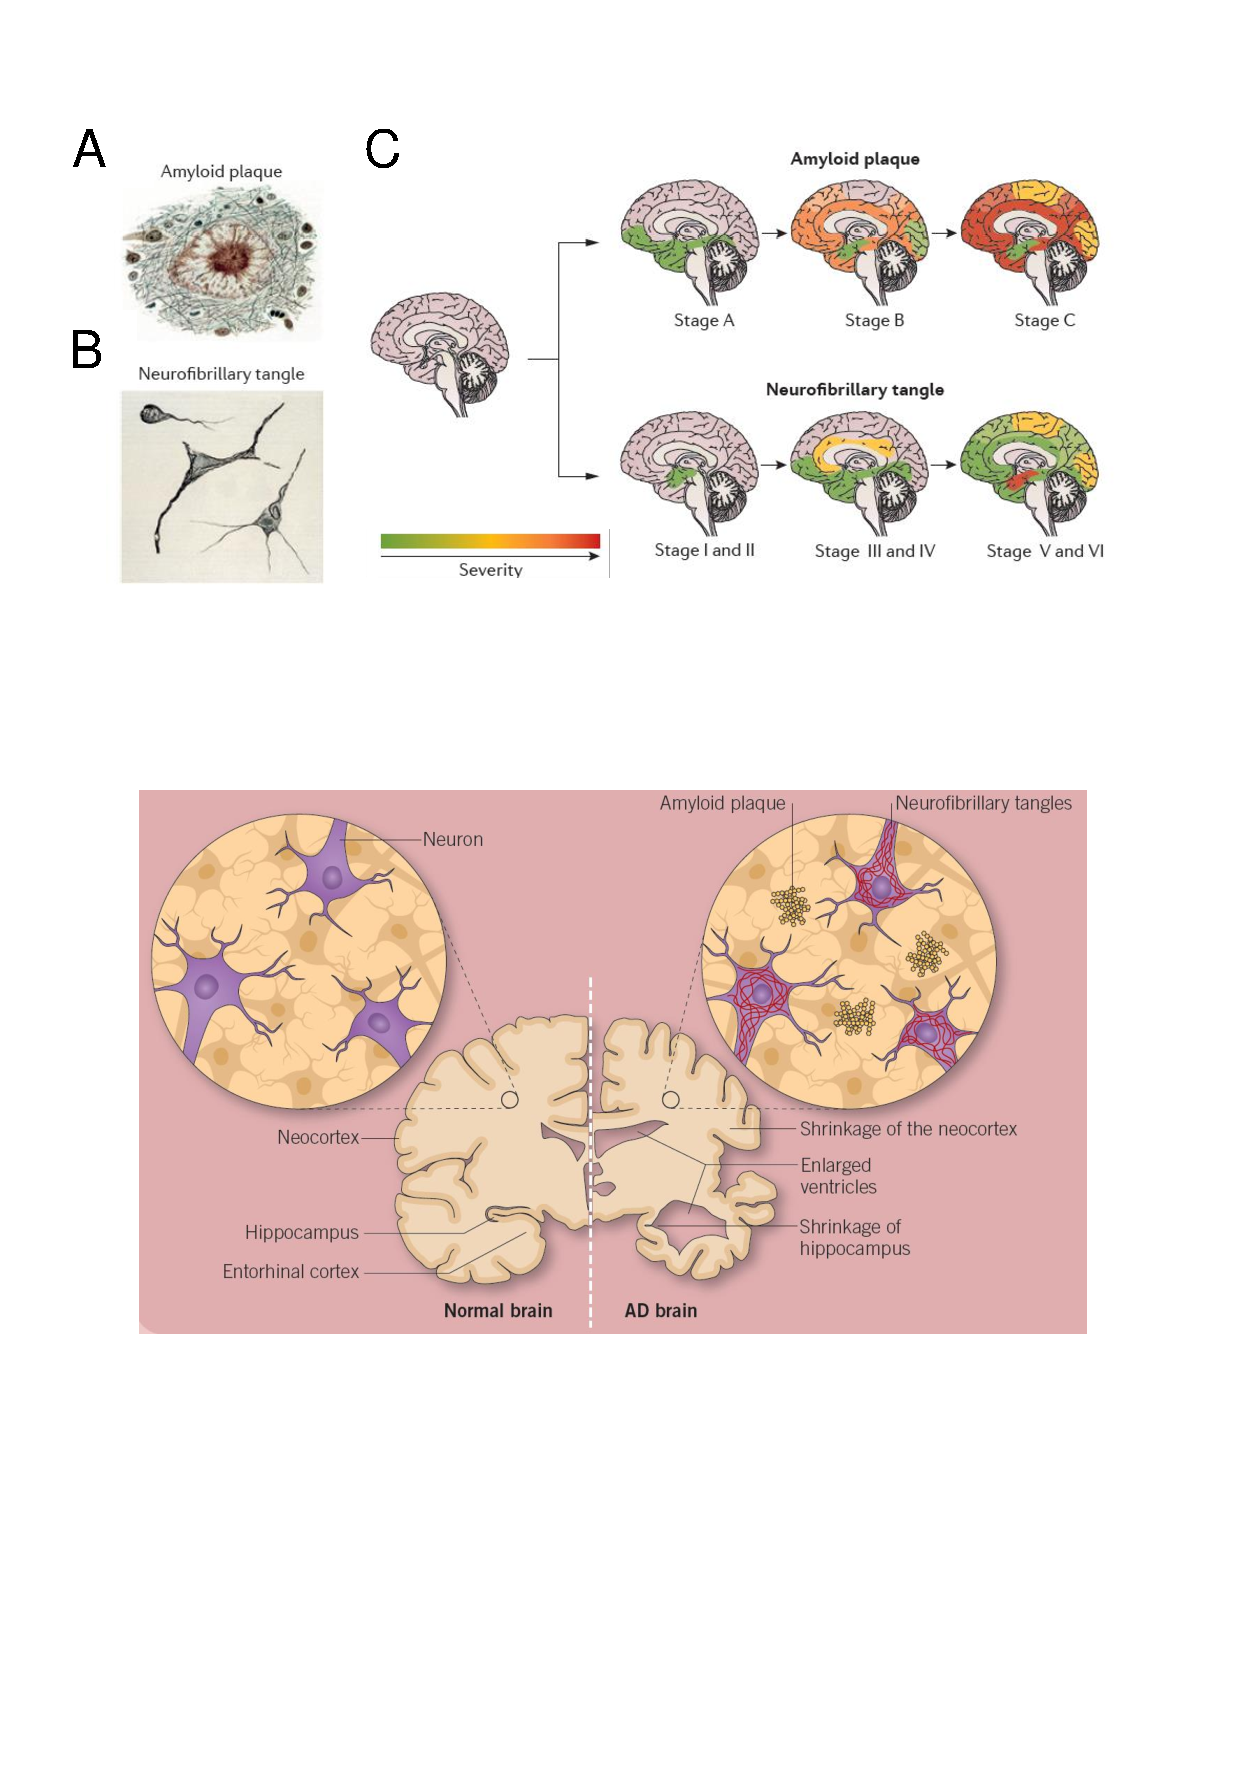
\includegraphics[page=1,trim={0 7cm 1cm 13cm},clip, scale = 0.75]{Figures/Introduction_Figures.pdf}
	\captionsetup{width=0.95\textwidth,singlelinecheck=off}
	\caption[Two key hallmarks of AD Neuropathology: amyloid plaques and neurofibrillary tangles]%
	{\textbf{Two key hallmarks of AD Neuropathology: amyloid plaques and neurofibrillary tangles.} A schematic comparing a normal healthy brain and a brain with advanced AD. AD pathology is well characterised by the presence of extracellular amyloid plaques and intracellular neurofibrillary tangles, accompanied by significant neuronal loss and subsequent shrinkage of the neocortex and hippocampus. Figure is taken from Palmer (2015)\cite{AlanM.Palmer2015}
	}
	\label{fig:AD_intro}
\end{figure} 

\begin{figure}[!htp]
	\centering
	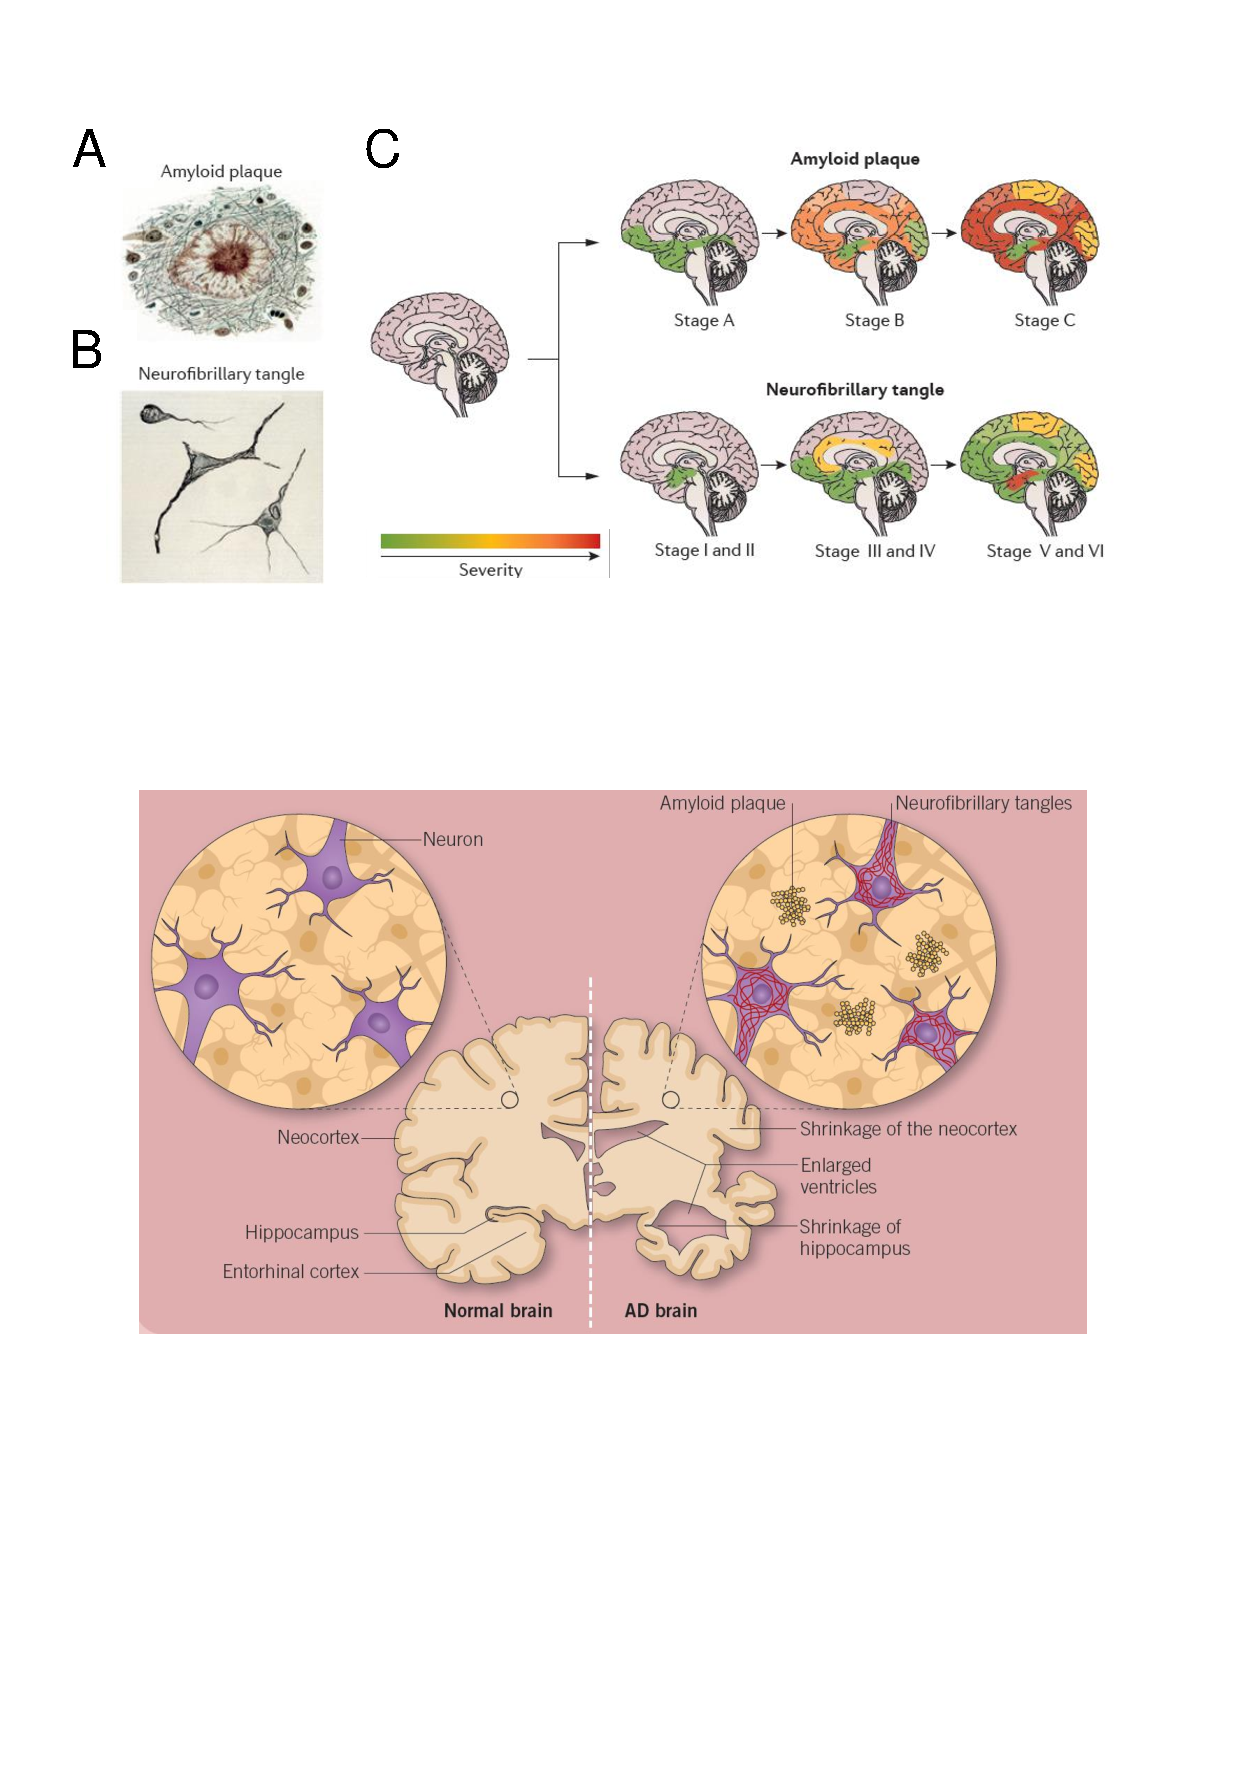
\includegraphics[page=1,trim={0 19cm 0cm 0cm},clip, scale = 0.8]{Figures/Introduction_Figures.pdf}
	\captionsetup{width=0.95\textwidth,singlelinecheck=off}
	\caption[Progression of amyloid plaques and neurofibrillary tangles with AD development]%
	{\textbf{Progression of amyloid plaques and neurofibrillary tangles with AD development.} Progression of \textbf{A)} amyloid plaques consisting of A$\beta$ measured according to Thal Phasing\cite{DR2002}, and \textbf{B)} neurofibrillary tangles composed of hyper-phosphorylated tau by Braak staging\cite{H1991}. Figure is taken from Masters et al. (2015)\cite{Masters2015}. 
		\\
		\\ 
		The deposition of A$\beta$ can be mapped Thal Phasing from the neocortex (Stage A), to b) allocortical regions comprising of the entorhinal cortex and hippocampus, the striatum (Stage B) and finally to iv) subcortical regions (Stage C)\cite{DR2002}. 
		\\
		\\
		In a similar pattern, the progressive spread of NFTs can be classified under the six stages of Braak from the trans-entorhinal regions such as the entorhinal cortex (Stage I,II), to the hippocampus (Stage III), adjoining neocortex (Stage IV) and finally to other neocortical regions (Stage V,VI)\cite{H1991}. 	
	}
	\label{fig:AD_development}
\end{figure}

\subsection{Genetics of AD}
Although AD predominantly affects people aged 65 and above (Late-Onset Alzheimer’s disease, LOAD\nomenclature{LOAD}{Late Onset Alzheimer's Disease}), 5\% of AD cases arise in much younger patients (Early-Onset Alzheimer’s disease, EOAD\nomenclature{EOAD}{Early Onset Alzheimer's Disease}). EOAD is typically associated with a clear familial autosomal dominant pattern of inheritance (Familial Alzheimer’s disease, FAD\nomenclature{FAD}{Familial's Alzheimer's Disease})\cite{Jarmolowicz2015}. To date, more than 160 highly-penetrant, causative mutations have been identified in EOAD, all located within three genes involved in A$\beta$ formation: \textit{APP} (amyloid precursor protein\nomenclature{APP}{Amyloid Precursor Protein}), \textit{PSEN1} and \textit{PSEN2} (presenilin 1 and 2\nomenclature{PSEN1}{Presenilin 1}\nomenclature{PSEN2}{Presenilin 2}) \cite{LM2010,Chai2007}. %While the clinical manifestations and presentation of neurological hallmarks are similar between EOAD and LOAD, patients with EOAD performed significantly worse in cognitive abilities not involved with memory (such as executive functions, language and visuoconstructional abilities)\cite{Joubert2016}.

While LOAD does not follow a typical Mendelian inheritance pattern, a relatively high heritability rate has been reported (50-80\% \cite{Gatz2006}), indicating that there is still a large genetic predisposition for developing AD in later years. Indeed, genome-wide association studies (GWAS\nomenclature{GWAS}{Genome-wide association studies}) and subsequent meta-analyses \cite{Bellenguez2020,Naj2020,Kunkle2019,Jansen2019,Lambert2013,Naj2011,Hollingworth2011,Harold2009,Lambert2009,Bertram2008} have identified over 75 genetic loci associated with an increased risk of developing LOAD. These GWAS loci are typically changes (or variants) at a single DNA base-pair (single-nucleotide polymorphisms – SNPs\nomenclature{SNP}{Single Nucleotide Polymorphism}) or small insertions and deletions (indels) that are found at a higher frequency in individuals with LOAD than in individuals without AD. 

The strongest genetic risk factor for LOAD to date is the $\epsilon$4 allele of \textit{APOE}\cite{Lambert2013}, the gene that encodes the cholesterol transporter apolipoprotein E (ApoE); this protein is a key regulator of lipid homeostasis, mediating lipid transport between astrocytes and neurons, a process critical for synaptic function and maintenance\cite{DH2001}. Harbouring one \textit{APOE}$\epsilon$4 allele increases the risk of developing LOAD by 3-4x, while harbouring two $\epsilon$4 alleles increases the risk by 15x\cite{Farrer1997}; conversely, the $\epsilon$2 allele is known to confer a neuroprotective effect against AD\cite{Nagy1995,EH1994}. Although the $\epsilon$4 allele is estimated to occur in \textasciitilde 15\% of the general population, it has been observed in 40\% of LOAD patients\cite{Farrer1997}. 

With the exception of \textit{APOE}, all the other GWAS-associated genetics variants are either common but lowly penetrant (i.e. SNPs annotated to \textit{CLU, PICALM}) or highly penetrant but rare (i.e. SNPs annotated to \textit{TREM2}) and collectively only contribute modestly to the risk of developing AD, highlighting the polygenic nature of AD (\cref{fig:AD_gwas}). While the molecular mechanisms through which these variants increase risk remain poorly understood, many are annotated to genes enriched in specific biological pathways (described in \cref{aetiologyAD}). 


\begin{landscape}
	\begin{figure}[!htp]
		\centering
		\includegraphics[page=11,trim={0 17cm 0cm 1cm},clip, scale = 1.2]{Figures/Introduction_Figures.pdf}
		\captionsetup{width=1.6\textwidth,singlelinecheck=off}
		\caption[Genetic landscape of AD]%
		{\textbf{Genetic landscape of AD.} Shown are the genes implicated in AD from the causative EOAD genes (\textit{APP, PSEN1, PSEN2}) identified from early family studies, to the GWAS-associated genes with either common but lowly penetrant variants or highly penetrant but rare variants. Variant penetrants, or effect size, is measured with the odds ratio (OR) with a larger odds ratio referring to a larger effect size. Variants conferring a protective and negative effect are denoted in orange and blue respectively. Figure was taken from DeRojas et al. (2021)\cite{DeRojas2021}. GWAS - Genome-wide association studies, OR - odds ratio
		}
		\label{fig:AD_gwas}
	\end{figure}
\end{landscape}

\subsection{Molecular mechanisms underlying AD pathogenesis}
\label{aetiologyAD}
Despite the fact that AD neuropathology has been well described (\cref{fig:AD_intro}), the exact biological mechanisms driving AD onset and pathogenesis are still widely unknown. To date, there are two key hypotheses proposed for the progression of AD: i) the amyloid cascade hypothesis, ii) the tau tangle hypothesis. Results from GWAS, however, implicate other pathways that could be involved including a dysfunctional immune response, lipid metabolism, endocytosis, and cell-adhesion molecule (CAM) pathways for synaptic signalling.  

\boldheader{Amyloid cascade hypothesis} 
The amyloid cascade hypothesis posits that the extracellular accumulation of A$\beta$ is the key driver of AD pathogenesis (\cref{fig:AD_development}\textbf{A}), which initiates a pathological cascade of NFT, cell loss and vascular damage \cite{Hardy1992}. A$\beta$ is comprised of short peptides (39-43 amino acids) \cite{J1987} produced from the amyloidogenic cleavage of APP (a transmembrane protein involved in synapse formation and stability) by $\beta$-secretase (BACE - β-site APP-cleaving enzyme 1\nomenclature{BACE}{Beta-secretase}) and $\gamma$-secretase (a complex protein consisting of PSEN1 and PSEN2) (\cref{fig:APP_Processing}). Due to cleavage at various sites, $\gamma$-secretase produces A$\beta$ of varying lengths, with 90\% secreted as A$\beta$\textsubscript{40} and the remaining 10\% as A$\beta$\textsubscript{42}\cite{Asami-Odaka1995}. In AD, the processing of APP is altered with the vast majority of causative \textit{APP}, \textit{PSEN1} and \textit{PSEN2} mutations favouring the production of the longer and more self-aggregating A$\beta$\textsubscript{42} \cite{Li2019,D1996,JT1993}, thereby promoting the formation of insoluble fibrils and plaques\cite{JT1993}. 

\begin{figure}[!htp]
	\centering
	\includegraphics[page=2,trim={0.5cm 9cm 0cm 15cm},clip, scale = 0.8]{Figures/Introduction_Figures.pdf}
	\captionsetup{width=0.95\textwidth,singlelinecheck=off}
	\caption[Sequential cleavage of APP into A$\beta$ by $\beta$-secretase and $\gamma$ secretase]%
	{\textbf{Sequential cleavage of APP into A$\beta$ by $\beta$-secretase and $\gamma$ secretase.}A schematic figure depicting sequential cleavage of APP, a transmembrane protein, either through the \textbf{A)} non-amyloidogenic pathway or the \textbf{B)} amyloidogenic pathway.
	\\
	\\
	In the non-amyloidogenic pathway, APP is cleaved by ADAM protein family (primarily, ADAM10, also known as $\alpha$-secretases) followed by $\beta$-secretase. Conversely in the amyloidogenic pathway, APP is sequentially cleaved by by $\beta$-secretase and $\gamma$-secretase, which produces A$\beta$ of varying lengths. Monomeric A$\beta$ molecules, particularly A$\beta$42, have increased propensity to oligomerise and aggregate to form the fibrils and plaques that are characteristic of AD. Figure is taken from Acker et. al (2019)\cite{Acker2019}. 
	}
	\label{fig:APP_Processing}
\end{figure}

\newpage
\boldheader{Tau tangle hypothesis} 
%https://pubmed.ncbi.nlm.nih.gov/33848474/
The tau tangle hypothesis posits that the phosphorylation and aggregation of tau to form NFTs are the primary drivers of AD\cite{KS1986} (\cref{fig:AD_development}\textbf{B}), which is also the defining feature of more than 20 other neurodegenerative disorders known collectively as tauopathies\cite{Orr2017}. Tau, encoded by the \textit{MAPT} gene, is a microtubule-associated protein involved in microtubule maintenance and stability. 

Recent studies suggest that tau is hyper-phosphorylated in AD, resulting in dissociation from microtubules and aggregation into filaments\cite{Grundke-Iqbal1986,Grundke-Iqbal1986a} (components of NFTs) that disrupt axonal transport and signal transmission, ultimately resulting in synpatic degeneration and loss\cite{Coomans2021} (\cref{fig:tau_hypothesis}). Tau mutations associated with frontotemporal dementia and parkinsonism (FTDP) \nomenclature{FTDP}{Frontotemporal dementia and parkinsonism} were found to induce conformational changes that increase the affinity for phosphorylation\cite{Alonso2004}. While no causative mutations in \textit{MAPT} have been identified in AD, the severity of NFTs has been shown to correlate better with cognitive decline and disease progression than amyloid plaques \cite{Serrano-Pozo2016,Giannakopoulos2003,PV1992}. Notably, regional variations in \textit{MAPT} transcript and protein expression were observed across the brain with a 2-fold increase in the neocortex compared to the cerebellum, potentially explaining the regional vulnerability of different brain regions to tau pathology\cite{Trabzuni2012}. 

\begin{figure}[!ht]
	\centering
	\includegraphics[page=13,trim={0 14cm 0cm 2cm},clip, scale = 0.6]{Figures/Introduction_Figures.pdf}
	\captionsetup{width=0.95\textwidth,singlelinecheck=off}
	\caption[Tau tangle hypothesis in AD]%
	{\textbf{Hyperphoshorylated tau dissociation from microtubules and aggregation into NFTs.} A schematic figure depicting \textbf{A)} a healthy neuron with normal tau and \textbf{B)} a diseased neuron with hyper-phosphorylated tau (orange spikes) detaching from microtubules, resulting in interrupted neuronal growth and function that is essential for synaptic transmission. Figure is taken from Brunden et al. (2009)\cite{Brunden2009}
	}
	\label{fig:tau_hypothesis}
\end{figure}	

\newpage
\boldheader{Endocytosis} 
Endocytic processing - the internalisation of substrates into the cell - is directly implicated in AD due to distinct cellular localisation of secretases involved in the amyloidogenic processing of APP\cite{Acker2019} (\cref{fig:APP_Processing}\textbf{B}). Contrary to the non-amyloidogenic pathway that predominantly occurs at the plasma membrane\cite{Sisodia1992} (\cref{fig:APP_Processing}\textbf{A}), amyloidogenic processing of APP takes place in the endosome and is spatially regulated: BACE1 and PSEN1/$\gamma$ complex are localised at the plasma membrane and thus must first undergo endocytosis before assemblage with PSEN2/$\gamma$ secretase at the endosome (\cref{fig:APP_Trafficking}). Increasing evidence suggests that regulation of this endocytic pathway is altered in AD, creating an intracellular pool of A$\beta$ peptides \cite{Peric2015} that coincide with cognitive deterioration in AD mouse models \cite{Tomiyama2010,Knobloch2007,Billings2005} and is more strongly associated to neuronal loss than A$\beta$ plaques\cite{Christensen2008}. Indeed, several risk genes emerging from recent GWAS are directly involved in endocytic regulation of APP processing, such as \textit{Bin1}, \textit{Picalm}, and \textit{Sorl1}\cite{Schmidt2016,Dumanis2015}(\cref{fig:APP_Trafficking}).   

\begin{figure}[!htp]
	\centering
	\includegraphics[page=6,trim={0 8cm 0cm 0cm},clip, scale = 0.7]{Figures/Introduction_Figures.pdf}
	\captionsetup{width=0.95\textwidth,singlelinecheck=off}
	\caption[Spatial regulation of APP trafficking and processing]%
	{\textbf{Spatial regulation of APP processing.} A schematic figure depicting APP trafficking and processing through the non-amyloidogenic (\cref{fig:APP_Processing}\textbf{A}), which predominantly occurs at the plasma membrane (boxed green), and amyloidogenic pathway (\cref{fig:APP_Processing}\textbf{B}), which preferentially occurs in the endosome (boxed red). APP processing through the amyloidogenic pathway is spatially regulated by the localisation and distinct internalisation of assembled PSEN1/$\gamma$ complex and BACE1 at the plasma membrane (boxed purple) and PSEN2/$\gamma$ in the endosome. Figure is adapted from Acker et. al (2019)\cite{Acker2019}  
	}
	\label{fig:APP_Trafficking}
\end{figure}

\newpage
\boldheader{Immune response}
Profound neuroinflammation - an inflammatory response within the CNS primarily orchestrated by the activation of microglia (microgliosis) and astrocytes (astrogliosis) - is widely implicated in AD development and pathology \cite{Cisbani2021,Griciuc2021}. While the exact role of the immune response is poorly understood in AD, it is widely accepted that an imbalance of the innate immune response is at play. This includes the extensive release of pro-inflammatory neurotoxic cytokines from activated microglia\cite{Frost2019} (\cref{fig:microglia_AD}\textbf{A}), which can trigger neuronal apoptosis\cite{Qin2002,Wang2015b} and β-secretase upregulation\cite{Chen2012}, resulting in enhanced A$\beta$ propagation (\cref{fig:microglia_AD}\textbf{B}). Furthermore, amyloid plaques were found enriched with activated microglia\cite{PL1987}, suggesting that plaque-associated microglia have a compromised phagocytic ability to remove A$\beta$\cite{Mawuenyega2010} - a complex process that involves recognition of toxic species by receptors (\cref{fig:microglia_AD}\textbf{B}) which have been previously identified in GWAS studies, such as TREM2, CD33 and CR1. 

\begin{figure}[!htp]
	\centering
	\includegraphics[page=8,trim={0 9cm 0cm 0cm},clip, scale = 0.8]{Figures/Introduction_Figures.pdf}
	\captionsetup{width=0.95\textwidth,singlelinecheck=off}
	\caption[Role of microglia in AD development and pathology]%
	{\textbf{Role of microglia in AD development and pathology.} A simplified schematic figure illustrating the \textbf{A)} multifaceted roles of microglia in AD, ranging from a protective to a detrimental role by the respective secretion of anti- and pro-inflammatory cytokines, and \textbf{B)} microglia's dual response to A$\beta$ plaques, either through A$\beta$ clearance or release of pro-inflammatory cytokines. Recent emergence of single RNA-sequencing studies have revealed significant heterogeneity in microglia isolated from AD post-mortem brain tissues, highlighting the complex role that microglia plays in AD development and pathology. Under physiological conditions, the microglia is ramified. PRR - Pattern recognition receptors, such as TREM2 and CD33, are found on the cell surface of microglia and are involved in recognising toxic species for phagocytosis. Both figures are adapted from Leng et al. (2021)\cite{Leng2021a}  
	}
	\label{fig:microglia_AD}
\end{figure}


\boldheader{Lipid metabolism}\label{intro_lipid}
Identification of \textit{APOE} $\epsilon$4 allele as the most robustly LOAD-associated genetic variant directly established a link between lipid metabolism and AD. Increasing evidence postulate that A$\beta$ clearance is regulated in an APOE isoform-dependent manner (ApoE2, ApoE3 and ApoE4)\cite{Castellano2011}, with ApoE4 having the lowest binding affinity to A$\beta$ and consequently, being the least efficient at A$\beta$ clearance compared to other ApoE isoforms\cite{RM2012}. The lipidation status of ApoE, mediated by ABCA1\cite{R2010}, is also known to impede A$\beta$ aggregation, with ApoE4 being the least lipidated\cite{DM2006}. Recent studies have further shown that A$\beta$ uptake is reduced in ApoE4-expressing microglia compared to ApoE3-expressing microglia, which is exacerbated upon Trem2 deficiency, revealing an interplay between lipid metabolism and immune response\cite{Fitz2021}. Notably, carriers of the $\epsilon$4 allele have more pervasive amyloid plaques than non-carriers\cite{DE1993,E2009}.

More broadly, lipid metabolism is implicated in AD development in that APP, $\beta$- and $\gamma$-secretase are all transmembrane proteins (\cref{fig:APP_Trafficking}). Consequently, APP trafficking and processing are influenced by lipid membrane constitution and organisation\cite{DiPaolo2011}; $\beta$-secretase activity is indirectly modulated by \textit{ABCA7}, which regulates the lipid membrane composition and is identified as a risk gene from GWAS studies\cite{Sierksma2020,Sakae2016}.  

%https://science.sciencemag.org/content/370/6512/61?rss=1

\clearpage
\subsection{Modelling AD: transgenic mouse models}
While profiling of human post-mortem brain tissues is typically considered the gold standard for studying AD pathogenesis, there are many limitations. Various confounding secondary factors (e.g. environmental exposures such as diet, medication) and technical difficulties (e.g. agonal state and post-mortem interval impacting RNA quality) all need to be considered. Given that the transcriptome from post-mortem tissues can only be evaluated at the time of death, it becomes challenging to resolve age-dependent and disease-associated changes. Conversely, mouse models of disease can be tightly controlled (i.e. genotype, living conditions, age and pathological status) to track progression of pathology in disease-relevant cell-types. As such, current mouse models act as a valuable reductionist tool to dissect the processes that drive the onset and progression of AD pathology, identify biomarkers and validate novel targets\cite{Hall2012}.

To study the different aspects of pathology, a number of transgenic AD mouse models have been developed with mutations that either result in amyloidopathy (A$\beta$ plaque formation) or tauopathy (NFT formation) (\cref{tab:mouse_models}). Amyloidopathy is typically developed through the insertion and overexpression of human \textit{APP}, either alone or in combination with \textit{PSEN1}, whereas tauopathy is recapitulated by overexpressing human \textit{MAPT} with FTD-associated mutations (given no causative \textit{MAPT} mutations have been identified in AD). 

\begin{table}[h]
	\centering
	\setlength\tabcolsep{3.5pt}
	\captionsetup{width=1\textwidth}
	\caption[Representative AD Mouse Models]%
	{\textbf{Representative AD mouse models}. Tabulated is a list of the most widely used AD mouse models developed from overexpression of one or more genes associated with FAD. Table is adapted from Hall et al. (2012) \cite{Hall2012} and is by no means comprehensive. mo - months}
	\label{tab:mouse_models}
	\begin{threeparttable}
		\begin{tabular}{@{}lllcccc@{}}
			\toprule
			\multicolumn{2}{c}{Mouse Models} &
			\multicolumn{1}{c}{Mutations} &
			\begin{tabular}[c]{@{}c@{}}Plaques\\  (mo)\end{tabular} &
			\begin{tabular}[c]{@{}c@{}}Tangles\\   (mo)\end{tabular} &
			\begin{tabular}[c]{@{}c@{}}Neuronal \\ Loss (mo)\end{tabular} &
			\begin{tabular}[c]{@{}c@{}}Cognitive \\ Deficit (mo)\end{tabular} \\ \midrule
			\multirow{4}{*}{hAPP}     & PDAPP                 & Ind\tnote{b}                        & 6  & x  & x     & 6                \\
			& Tg2576                & Swe\tnote{a}             & 11 & x  & x     & \textgreater{}12 \\
			& J20                   & Swe\tnote{a}, Ind\tnote{b} & 6  & x  & x     & 4                \\
			& APP23                 & Swe\tnote{a}               & 6  & x  & 14-18 & 3                \\
			\multirow{3}{*}{hAPP/PS1} & PS/APP & Swe\tnote{a}, M146L\tnote{e}                 & 6  & x  & 22    & 3                \\
			& APP/PS1         & Swe\tnote{a}, PSEN1dE9              & 6  & x  & x     & 6                \\
			& 5xFAD                 & Swe\tnote{a}, Lon\tnote{a}, Flo\tnote{c}, M146L\tnote{e}, L28V\tnote{e} & 2  & x  & 9     & 4                \\
			\multirow{4}{*}{hTau}     & hTau.P301S            & MAPT P301S                 & x  & 4  & 3     & 3                \\
			& 3xTg                  & Swe\tnote{a}, MAPT P301L, M146V     & 6  & 12 & -    & 4                \\
			& rTg4510               & MAPT P301L                 & x  & 4  & 6     & 3                \\
			& htau                  & Wildtype                   & x  & 9  & 10    & 6                \\ \cmidrule(l){1-7} 
		\end{tabular}
		\begin{tablenotes}
			\footnotesize
			\item[a] Swedish APP mutation K670N/M671L
			\item[b] Indiana APP mutation V717F
			\item[c] London APP mutation V717I
			\item[d] Florida APP mutation I716V 
			\item[e] Human PSEN1 mutations 
		\end{tablenotes}
	\end{threeparttable}
\end{table}

It is also important to note that there is currently no AD mouse model that encapsulates all the defining features of AD, and one of the major criticisms of current mouse models relates to how representative they are of sporadic, late-onset AD. The insertion of transgenes is also found to disrupt endogenous mouse genes that may significantly contribute to the neurodegenerative phenotype observed in these mice\cite{Gamache2019}. While there have been recent efforts to generate mouse models that more closely resemble LOAD with the incorporation of AD-associated variants, such as the \textit{APOE} $\epsilon$4 variant \cite{apoe4trem2_mousemodel,Lewandowski2020}, these models are not widely used. 

Nonetheless, a recent meta-analysis of differential expression studies in human post-mortem samples revealed that many transgenic mice display gene expression signatures that significantly overlap with human AD-associated co-expression modules, particularly neuronal and microglia-enriched modules\cite{Wan2020}. While they concluded that there is a minority of human AD-associated co-expression modules that were poorly recapitulated by current AD mouse models (such as genes involved in proteostasis regulation), they highlighted the utility of mouse transcriptomic data from multiple time points to accelerate discovery of AD progression markers and identify critical time-points for interventions; memory task impairment and neurodegenerative pathology of rTg4510 transgenic mice at 4 and 6 months were found to correspond to activation of the neuronal and microglial expression pattern, respectively. 

In my thesis, I utilise the rTg4510 mouse model at 4 different ages (2, 4, 6 and 8 months) to profile progressive transcriptomic changes associated with development of tau pathology. The range of age selected reflect the development of age-dependent tauopathy in these mice from 

Overexpressing the human tau transgene, rTg4510 transgenic mice develop age-dependent tauopathy with pretangles observed as early as 3 months, synaptic and neuronal loss by 6 and 9 months respectively. These mice further display behavioural More details on this model are provided in \cref{ch: general methodology}. 


\clearpage
\section{Transcriptional dysregulation in AD}

The vast majority of GWAS variants associated with LOAD are annotated to non-coding regulatory regions of the genome and are enriched in open chromatin regions that promote transcription such as enhancers\cite{Kikuchi2019} (short DNA sequences containing specific motifs for binding of transcription factors), suggesting that AD-associated risk variants mediate disease associations through gene transcriptional regulation. As such, efforts have been made in profiling the complete set of expressed messenger RNA (mRNA\nomenclature{mRNA}{Messenger RNA}) transcripts (hereby referred as transcriptome) in AD mouse models and post-mortem brain tissues to better understand the expression changes underlying AD pathogenesis. 

A number of studies have identified widespread gene differences in human AD post-mortem brain tissues (reviewed in \cref{tab: AS_ADHuman_studies}) and in transgenic mice harbouring AD-associated mutations (reviewed in \cref{tab: AS_ADMouse_studies}). Recent works in our group have similarly identified robust changes in gene expression associated with tau pathology development in rTg4510 transgenic mice, with these genes enriched in biological pathways previously implicated in AD pathology\cite{Castanho2020}. 

However, one major limitation of these studies is that they have broadly ignored identifying differences at the RNA transcript level, given that efforts to perform these analyses up until now have largely been hampered by technology (more details to follow in \cref{rnaseq_intro}). Deeper examination and investigation of changes at the transcript level will be critical, particularly since changes at the transcript level do not necessarily translate to changes at the gene level - expression of transcripts in opposite directions may result in zero net change at the level of gene expression. Transcriptomic profiling of disease-relevant tissues to examine whether specific transcripts are altered in AD would therefore be pertinent, especially given that there is an increasing interest in the role of aberrant alternative splicing in Alzheimer's disease \cite{Raj2018}.

\subsection{Alternative Splicing}\label{intro:AS}
Alternative splicing is a transcriptional regulatory mechanism that produces distinct RNA transcripts (isoforms) from a single gene, which are potentially translated to different protein isoforms with unique, and potentially, antagonistic functions\cite{Wang2008}. It is a widespread phenomenon with over 95\% of human genes estimated to be influenced \cite{Pan2008}, and is most prevalent in the brain\cite{Yeo2004}, where it impacts upon neuronal development and maintenance\cite{Pan2008, Mazin2014, Raj2015}. There is a growing recognition of the key role of aberrant mis-splicing in neurodegenerative diseases \cite{Gandal2018,RL2019}, including schizophrenia and autism. 

\boldheader{Mechanism}
Splicing involves the removal of non-coding sequences (introns) from mRNA precursors and the ligation of coding sequences (exons), resulting in isoforms with different exonic structures (\cref{fig:AS_events}). This relies on the concerted and regulated assembly of the spliceosome - a multimegaton, dynamic ribonucleoprotein complex - by its recognition and stepwise-binding to sequence elements within the pre-mRNA (cis-acting elements), and a group of RNA-binding proteins (trans-acting splicing factors) (\cref{fig:AS_mechanism}). This process is highly regulated in a temporal and cell-specific manner, and requires multiple components at work, including i) the sequence of cis-acting elements within the exon or intron, which determines the binding affinity of splicing factors that either enhance or suppress splicing, ii) the availability of such splicing factors, and iii) the functional coupling of transcription and splicing, mediated by epigenetics, chromatin and RNA structure, and iv) polymerase processivity and elongation rate.
%There are two types of spliceosome - major and minor - both of which involve the activity of five uridine-rich small nuclear ribonucleoproteins (snRNP\nomenclature{snRNPs}{Small Nuclear Ribonucleoproteins}) and numerous non-snRNP proteins\cite{Will2011}. Using a similar mechanism but composed of different snRNPs, the minor spliceosome removes less than 1\% (0.4\%) of introns\cite{Turunen2013} and is thus referred to as "U12-dependent non-canonical splicing", as opposed to "U2-dependent canonical splicing" with major spliceosome.


\begin{figure}[!h]
	\centering
	\includegraphics[page=9,trim={0 16.5cm 0cm 0},clip, scale = 0.7]{Figures/Introduction_Figures.pdf}
	\captionsetup{width=0.95\textwidth,singlelinecheck=off}
	\caption[Alternative Splicing Events]%
	{\textbf{Alternative Splicing Events.} Splicing involves removal of introns and ligation of exons either constitutively or alternatively to generate isoforms with different exonic structure from i) exclusion of an entire exon (orange exon in SE), ii) mutual exclusion of two exons (orange and blue exons in MX) ii) inclusion of an intronic sequence (light orange in IR), iii, iv) usage of a different 5'SS or 3'SS resulting in a novel splice junction (A5', A3') and the v, vi) usage of different first and last exons which can result in an alternative initiation and termination sites. Introns and exons are depicted by the box and line respectively. 
	}
	\label{fig:AS_events}
\end{figure}

Correct splicing first requires recognition of short sequence motifs upstream (5' splice site, 5'SS\nomenclature{5'SS}{5' Splice Site}, donor site) and downstream (3' splice site, 3'SS\nomenclature{3'SS}{3' Splice Site}, acceptor site) of the intron/exon boundary (splice junctions) (\cref{fig:AS_mechanism}\textbf{A}),  followed by sequential assembly of the spliceosome components and intron excision\cite{Herzel2017}(\cref{fig:AS_mechanism}\textbf{B}). The 5'SS is typically defined by a conserved 9-nucleotide sequence with a GU(T) dinucleotide, and the 3'SS by a polypyrimidine tract (PPT\nomenclature{PPT}{Polypyrimidine Tract}) followed by a conserved AG dinucleotide \cite{Will2011}. Almost all introns in human and mouse are flanked by the GT-AG splice site dinucleotide\cite{Sheth2006}, with other dinucleotide variations known to exist in very minute proportions: GC-AG and AT-AC comprises \textasciitilde0.9 and \textasciitilde0.09\% of human splice sites respectively\cite{Parada2014}. An increasing number of diseases are linked to aberrant alternative splicing predominantly by the presence of pathogenic variants disrupting the cis-acting elements and interfering with the functional activity of trans-acting protein splicing factors; variations in 5'SS and 3'SS can result in exon skipping, exon inclusion, exon extension or exonic splice gain whereas variations in intron result in intron gain.

\begin{figure}[!htp]
	\centering
	\includegraphics[page=3,trim={0 14cm 8cm 2cm},clip, scale = 0.8]{Figures/Introduction_Figures.pdf}
	\captionsetup{width=0.95\textwidth,singlelinecheck=off}
	\caption[Splicing Mechanism: spliceosome assembly on nascent RNA]%
	{\textbf{Intron removal is catalysed by the assembly and complex rearrangement of the spliceosome. a)} The consensus sequence of the splice junctions that demarcate the intron/exon boundary and are essential for recruitment of spliceosomal snRNPs (small nuclear ribonucleoproteins). \textbf{B)} Co-transcriptional assembly of spliceosome with stepwise interaction of spliceosomal snRNPs, with the formation of 
		\begin{enumerate}
			\item E (Early) commitment complex with the identification and binding of U1 snRNP to the 5'SS and branchpoint binding protein (BPP) to BPS 
			\item A (Assembly) catalytically-active complex with association of U2 snRNP to the branch site following the dissociation of BPP. The "A" here denotes the adenosine of BPS
			\item B pre-catalytic spliceosome complex with recruitment of U4,U5 and U6 snRNPs
			\item B pre-catalytic spliceosome complex after major conformational rearrangements within the spliceosome (RNA-protein and RNA-RNA interactions) followed by the release of U1 and U4 snRNP to expose the adenosine from BP to the 5'SS 
			\item B* catalytically-active complex with nucleophilic attack of adenosine on 5'SS (1st step of transesterification) 
			\item C catalytically-active complex with further conformational changes of the U2 snRNP to C* complex, with nucleophilic attack of the 5'SS to 3'SS (2nd step of trans-esterification) 
			\item P (Post-spliceosome complex) with release of the mRNA transcript from the remaining spliceosome (ILS), now bound to the intron lariat. The snRNPs are then disassociated and recycled for the next cycle of splicing.
			\\
		\end{enumerate} 
		Intron excision is primarily executed by two transesterification reactions. BBP - Branchpoint Binding Protein, BPS - Branch Point Sequence, CTD - Carboxyl-terminal Domain, ILS - Intron Lariat Spliceosome, PAS - Poly(A) Site, SS - Splice site, SnRNP - Small nuclear ribonucleoproteins, \nomenclature{TSS}{Transcription Start Site}, TTS - Transcription Termination Site\nomenclature{TTS}{Transcription Termination Site}. Figure is taken from Herzel et al. 2017\cite{Herzel2017}.
	}
	\label{fig:AS_mechanism}
\end{figure}

\vspace{1.5cm}
\boldheader{Nonsense-mediated decay}
Up to one-third of alternative splicing events introduce premature termination codons (PTCs) that are typically located > 50- 55 nucleotides upstream of splice junction, leading to premature mRNA degradation - a process known as Nonsense mediated decay (NMD)\cite{Lewis2003} \nomenclature{NMD}{Nonsense Mediated Decay}. While NMD was initially considered an RNA surveillance mechanism involved in removing unproductive and detrimental slice variants, it is now widely acknowledged as a key mechanism for gene regulation\cite{Nickless2017} - up to 25\% of naturally-occurring transcripts are estimated to be affected\cite{Weischenfeldt2012}. Notably, intron-retaining transcripts often contain a PTC, implicating the coupling of intron retention events to NMD\cite{Wong2013}.     

\newpage
\subsection{Other regulatory mechanisms}
Adding to the layer of complexity are other alternative RNA processing regulatory mechanisms that regulate gene expression, such as alternative transcription initiation (ATI \nomenclature{ATI}{Alternative Transcription Initiation}) with alternative promoter usage and alternative transcription termination (ATT\nomenclature{ATT}{Alternative Transcription Termination}) sites with alternative polyadenylation (\cref{fig:AS_others}). More than 70\% of mammalian genes are reported to contain multiple polyadenylation sites and 60\% with two or more promoters from alternative transcription start sites\cite{Carninci2006}. Alternative transcription at these sites generate RNA isoforms with different 3' and 5' untranslated regions (UTRs) that may translate to proteins with varying 5'/3' terminals. Importantly, introduction of variable UTRs can further modulate transcription regulation by fine-tuning the mRNA stability, localisation and translation efficiency\cite{Reyes2018}. This is in contrast to alternative splicing where changes typically lie within the protein sequence, which could potentially influence protein structure and function.

\begin{figure}[!h]
	\centering
	\includegraphics[page=14,trim={0 15cm 2cm 2cm},clip, scale = 0.7]{Figures/Introduction_Figures.pdf}
	\captionsetup{width=0.95\textwidth,singlelinecheck=off}
	\caption[Alternative transcription coupled with Alternative Splicing Mechanisms]%
	{\textbf{Alternative Transcription mechanisms to regulate gene expression.} A schematic figure depicting the gene locus and associated isoforms, generated from alternative splicing (AS) and other alternative transcription mechanisms in the 5' and 3' end: Alternative transcription initiation (ATI), Alternative transcription termination (ATT). \newline
	TI - Transcription initiation site, TS - Translation initiation site, TT - Transcription termination site; * - translation termination site. Protein-coding regions are filled. Frequent alternative exons (AEs) and common combinations of AEs are shown in red. Rare AEs and avoided combinations of AEs are shown in blue. Figure and legend is adapted from Shabalina et. al (2010)\cite{Shabalina2010}
	}
	\label{fig:AS_others}
\end{figure}

\newpage
\subsection{Crosstalk between Epigenetics and Alternative Splicing}
Epigenetics typically refer to the heritable, but reversible, alterations to the chromatin structure that can dynamically influence gene expression in a temporal and cell-type-specific manner. These alterations are broadly recognised into two groups\cite{Docherty2008}: i) chemical modifications of the DNA base, with methylation (addition of a methyl group to the cytosine in CpG dinucleotides, resulting in 5'mC) as the most stable modification, or ii) post-translational modifications of histone proteins, the basic proteins around which DNA is wrapped for tight packaging into chromatin.      

DNA methylation at promoters regions enriched with CpG sites has been heavily associated with chromatin repression and subsequent gene silencing. While the function of DNA methylation in gene body remains elusive, reports have shown that gene body DNA methylation can influence polymerase processivity and elongation rate \cite{Yang2014}, which can in turn determine the splicing of weak alternative exons. Recent studies have further identified splicing regulatory factors whose splicing activity is influenced by DNA methylation\cite{Shukla2011}. One such example is CTCF, where DNA methylation inhibits its binding to \textit{CD45} exon 5, thereby enabling Polymerase II to transcribe more rapidly and subsequently result in exclusion of exon 5\cite{Shukla2011}. Notably, various histone modifications have also been shown to influence splicing by impacting the recruitment of splicing factors\cite{Zhang2020a, Luco2011}.

\newpage
\subsection{Altered splicing in AD}\label{intro:AD_alteredsplicing}
Aside from extending the diversity of the transcriptome and proteome, alternative splicing offers an additional regulatory level of protein homeostasis in addition to transcription and translation. Dysregulation of splicing can have significant functional consequences in driving or contributing to disease progression and susceptibility, by disrupting protein isoform function (loss-of-function or gain-of-function) or generating an imbalanced isoform ratio (i.e. a change in relative isoform expression). Studies on the role of alternative splicing in AD have largely focused on identifying mis-splicing variants of FAD genes; such as the \textit{PSEN1} intron 4 mutation which generates aberrantly-spliced PSEN1 isoforms that were found to increase A$\beta$42 \textit{in vitro}\cite{DeJonghe1999}. Perhaps more well known is the altered splicing of \textit{MAPT} whereby exclusion or inclusion of exon 10 (E10) generates isoforms with either 3 (3R tau, E10-) or 4 (4R tau, E10+) microtubule-binding repeat domains, with the latter having a greater interaction with microtubules. Over 50 tauopathy-associated intronic mutations were found clustered around the 5'SS of exon 10, favouring exon 10 inclusion \cite{DSouza1999, Ghetti2015} and leading to an increased 4R/3R ratio that contributes to tau aggregation \cite{Adams2010}. Mimicking this imbalanced ratio in a tauopathy mouse model induced more phosphorylated,self-aggregating tau and seizures\cite{Schoch2016}.  

Notably, multiple spliceosomal components were found to co-aggregate with tau in human AD post-mortem brain tissues\cite{Bai2013}, implicating a global change in the core splicing machinery and disruption of splicing in AD pathogenesis. Recent transcriptomic profiling of various human AD post-mortem brain regions (reviewed in \cref{tab: AS_ADHuman_studies}) and AD mouse models (reviewed in \cref{tab: AS_ADMouse_studies}) have revealed aberrant splicing as a hallmark of AD. Hundreds of genes have been reported to be differentially spliced with widespread transcript expression differences and usage of alternative splicing events in genes such as \textit{APOE, BIN1} and \textit{APP}\cite{Marques-Coelho2021, Raj2018}. Furthermore, these AD-associated splice variants (splicing quantitive trait loci - sQTL) were enriched in transcriptionally active regions that overlap with other AD-associated SNPs and epigenetic variants, highlighting the genomic complexity underlying AD pathogenesis.  

\begin{changemargin}{1.5cm}
	%\captionsetup{width=30cm}
	\begin{landscape}
		\small %smaller font
		\setlength\tabcolsep{2pt} %reduced margin size in table
		\renewcommand{\arraystretch}{1}
		\begin{longtable}[c]{p{3cm}p{4cm}p{3cm}p{16cm}}
			\caption[Transcriptomic studies in AD human post-mortem brain tissues]%		
			{\textbf{Transcriptomic studies in AD human post-mortem brain tissues reveal mis-splicing as a widespread hallmark of AD}. \newline AS - Alternative Splicing, hnRNP - Heterogeneous nuclear Ribonucleoproteins, IR - Intron Retention, LOF - Loss-of-Function, NMD - Nonsense-mediated mRNA Decay, qPCR - quantitative Polymerase Chain Reaction, RBP - RNA Binding Protein, RNA-Seq - RNA-Sequencing, snRNP - Small nuclear Ribonucleoproteins, SE - Skipped Exon, TSS - Transcription Start Site, TWAS - Transcriptome-wide Association Studies}
			\label{tab: AS_ADHuman_studies}\\
			
			\toprule
			\multicolumn{1}{c}{References} &
			\multicolumn{1}{c}{Samples and Tissues} &
			\multicolumn{1}{c}{Method} &
			\multicolumn{1}{c}{Key Findings} \\* \midrule
			\endfirsthead
			%
			\endhead
			%
			\bottomrule
			\endfoot
			%
			\endlastfoot
			%		
			\centering Twine et al. (2011)\cite{Twine2011} &
			\centering 3 AD, 33 Controls\newline Total, frontal \& temporal lobe &
			\centering RNA-Seq &
			\tabitem \textit{APOE} was downregulated in AD temporal lobe. Identified 3 isoforms with different TSS and isoform expression: ENST00000252486 and ENST00000446996 from TSSA were downregulated (3.09-fold) whereas ENST00000425718 from TSSB was upregulated (26.5-fold) \newline
			\tabitem \textit{Ank1} was downregulated in AD total brain \\
			\hdashline[0.5pt/5pt]
			
			\centering Mills et al. (2013)\cite{Mills2013} &
			\centering 5 AD, 5 Controls \newline Parietal lobe &
			\centering RNA-Seq &
			\tabitem Differentially expressed genes were enriched in lipid metabolism (\textit{ACOT1}, \textit{ACOT2} and  \textit{DBI/ACBP} was upregulated, whereas \textit{TECR} was downregulated) \newline
			\tabitem Differential isoform expression observed in \textit{DBI/ACBP}: non-coding DBI-009 was upregulated while protein-coding DBI-003 was downregulated. \\
			\hdashline[0.5pt/5pt]
			
			\centering Bai et al. \newline(2013)\cite{Bai2013} &
			\centering 18 AD, 17 Controls \newline Cortex &
			\centering Mass Spectrometry, RNA-Seq &
			\tabitem Extranuclear aggregation of 36 proteins, including spliceosomal components (U1 snRNP, U1-70K) \newline
			\tabitem Accumulation of unspliced RNA molecules in AD, with reduced splicing efficiency (increased ratio of pre- and mature RNA) in AD-associated genes (\textit{BACE1, BIN1, CLU, GFAP, PICALM, PSEN1, SORL1})  \\
			\hdashline[0.5pt/5pt]
			
			\centering  Lai et al. \newline(2014)\cite{Lai2014} &
			\centering 8 AD, 8 Controls\newline Superior Temporal Gyrus &
			\centering Microarray &
			\tabitem 22 genes identified with differential AS events (characterised by differential exon usage) \newline  
			\tabitem \textit{GNAL} transcript variant 5 downregulated in AD whereas transcript variant 1 showed no change \newline 
			\tabitem \textit{MAP4} transcript variant 3 downregulated in AD whereas transcript variant 1 was upregulated\\
			\hdashline[0.5pt/5pt]
			
			\centering Mills et al. (2014)\cite{Mills2014} &
			\centering 14 AD, 16 Controls \newline Superior Temporal Gyrus &
			\centering RT-qPCR &
			\tabitem No difference in total \textit{APOE}, \textit{APOE-005}, or \textit{APOE-001} expression between AD superior temporal gyrus and controls, contrary to Twine et al. (2011)\cite{Twine2011} \\
			
			\centering Humphries et al.(2015)\cite{Humphries2015} &
			\centering 10 AD, 10 Controls, \newline Temporal lobe &
			\centering RNA-Seq &
			\tabitem 9 genes were differentially expressed (i.e. \textit{ABCA7, CR1}), 5 of which had differential splicing (\textit{ABCA7, TMEM259, EPHA1, MS4A6A, MS4A6E}) defined by differences in overall exon distribution \\
			\hdashline[0.5pt/5pt]
			
			\centering Magistri et al.(2015)\cite{Magistri2015} &
			\centering 4 AD, 4 Controls \newline Hippocampus &
			\centering RNA-Seq &
			\tabitem Downregulation of \textit{TAC1} and upregulation of \textit{SERPINE1} \newline 
			\tabitem Pathway analysis indicates dysregulation in neural communication and A$\beta$ clearance \\		
			\hdashline[0.5pt/5pt]
			
			\centering Alkallas et al. (2017)\cite{Alkallas2017} &
			\centering 6 AD, 5 Controls \newline Dorsolateral Cortex &
			\centering RNA-Seq &
			\tabitem RBFOX1 (RBP) is downregulated in AD; reduced stability and abundance of RBFOX-regulated transcripts that encode synaptic transmission proteins, contributing to loss of synaptic function	\\
			\hdashline[0.5pt/5pt]
			
			\centering Annese et al. (2018)\cite{Annese2018} &
			\centering 6 AD, 6 Controls \newline Hippocampus, Temporal and Frontal lobe &
			\centering RNA-Seq &
			\tabitem 2,122 differentially expressed genes, including upregulation of \textit{TESPA1, CPLX3 SERPINA5, SERPINA1} and dowregulation of \textit{NEUROD6, NEUROD1, LOC400891, CAMK1D} \newline
			\tabitem Deregulated micro-RNA (miR-132/212) and general decrease in RNA editing in AD \\
			\hdashline[0.5pt/5pt]
			
			\centering Raj et al. \newline (2018)\cite{Raj2018} &
			\centering 268 AD, 182 Controls \newline Dorsolateral prefrontal cortex &
			\centering RNA-Seq &
			\tabitem 84 differentially spliced genes defined by differential intron usage, 11 of which also differentially expressed (\textit{PFKP, NDRG, APP, PICALM, CLU}) \newline
			\tabitem sQTLs enriched in RBPs, including \textit{PTBP1, ELAVL1} and multiple hnRNPs \newline
			\tabitem TWAS identified 21 genes with differential intron usage associated with AD, including \textit{CR1,PTK2B, CLU, AP2A1, AP2A2, MAP1B} \\
			\hdashline[0.5pt/5pt]
			
			\centering Johnson et al. \newline (2018)\cite{Johnson2018} &
			\centering 20 AD, 13 Controls \newline Dorsolateral prefrontal cortex &
			\centering Mass-Spectrometry &
			\tabitem More alternative exon-exon junction peptides mapped to \textit{MAPT, BIN1, PTK2B, FERMT2} in AD. \newline 
			\tabitem Higher RBPs protein levels detected in AD, with enrichment in modules correlated with tau pathology \\
			\hdashline[0.5pt/5pt]	
			
			\centering Han et al. (2019) \cite{Han2019} &
			\centering 24 AD, 50 Controls \newline Hippocampus &
			\centering RNA-Seq &
			\tabitem 3 AD-associated SE events in \textit{RELN} \& \textit{NOS1}, resulting in truncated proteins with loss of functional domains. A SNP was identified adjacent to \textit{RELN} skipped exon \& within splicing regulatory element. \\
			
			\centering Adusumalli et al. (2019) \cite{Adusumalli2019} &
			\centering 4 2AD, 38 Controls\cite{Bai2013} \newline Frontal cortex &
			\centering Mass Spectrometry &
			\tabitem 1,136 differential IR events annotated to 781 genes (including \textit{BIN1, MAPT}), which were enriched in mRNA export and splicing, and had significantly different protein levels between AD and controls \newline
			\tabitem Differentially retained introns have higher GC content, suggesting that DNA methylation changes may contribute to differential IR \\
			\hdashline[0.5pt/5pt]
			
			\centering Fan et al. (2021) \cite{Fan2021} &
			\centering 210 AD, 191 Controls\textsuperscript{a} &
			\centering RNA-Seq &
			\tabitem 2 isoform modules with 38 isoforms upregulated in AD, 33 of which has not been reported as AD-associated (including \textit{ANLN, DOCK5, ERBB3, SEPT8, UGT8}). 67 genes were identified with differentially expressed isoforms in different modules  \\
			\hdashline[0.5pt/5pt]
			
			\centering Yang et al. (2021) \cite{Yang2021} &
			\centering 1074 AD, 608 Controls \newline 9 brain regions&
			\centering RNA-Seq & 
			\tabitem 1,530 differential SE events in 1,103 genes enriched in endocytosis; 2,415 differential SE events in 1,701 genes associated with tau progression and enriched in axon guidance \newline 
			\tabitem \textit{MBP} exon 5 skipping; \textit{ASPH} exon 5 and exon 8 skipping in cerebellum \newline  
			\tabitem 15,556 ES events in 113 RBP (\textit{CHL1} exon 25, \textit{ASPH} exon 5); \textit{RBM3, RBPMS2, AZGP1, RPS16} were differentially expressed in STG; SNP in \textit{ABCA7} donor site was associated with exon 2 skipping \newline 
			\tabitem 70\% of genes predicted LOF due to SE, with most significant loss attributed to peptidy-serine phopshorylation; 86 AD genes with partial function loss were enriched in neuronal development	\\
			\hdashline[0.5pt/5pt]		
			
			\centering Garcia-Escudero et al. (2021) \cite{Garcia-Escudero2021} &
			\centering 32 AD (Braak I-VI), 10 Controls &
			\centering qPCR, Western Blot &
			\tabitem Identified novel human-specific truncated Tau isoform with intron 12 retention, which is downregulated in AD and is less prone to aggregate compared to other tau isoforms \\
			\hdashline[0.5pt/5pt]
			
			\centering Li et al. (2021) \cite{Li2021} &
			\centering 84 AD, 80 Controls \newline Temporal cortex &
			\centering RNA-Seq, Mass Spectrometry &
			\tabitem Higher intron-retained levels in AD (including \textit{BACE1, BIN1, PICALM}) but no differential gene expression, suggesting a compensatory mechanism \newline
			\tabitem HMBOX1, a transcription factor involved in innate immune response, had the strongest  differentially expressed intron level associated with tau pathology \newline
			\tabitem Increased IR was associated with reduced protein expression, possibly due to NMD \\* \bottomrule
		\end{longtable}

		\begin{longtable}[c]{p{3cm}p{4cm}p{3cm}p{16cm}}
			\captionsetup{width=1.6\textwidth}
			\caption[Transcriptomic studies in AD mouse models]%		
			{\textbf{Transcriptomic studies in AD mouse models reveal mis-splicing as a widespread hallmark of AD}. \newline AS - Alternative Splicing, hnRNP - Heterogeneous nuclear ribonucleoproteins, FAD - Familial Alzheimer's Disease, GWAS - Genome-wide Association Studies, NFT - Neurofibrillary Tangles, NMD - Nonsense-mediated mRNA Decay, RBP - RNA binding protein, RNA-Seq - RNA-Sequencing, TG - Transgenic}
			\label{tab: AS_ADMouse_studies}\\
			\toprule
			\multicolumn{1}{c}{References} &
			\multicolumn{1}{c}{Mouse Models \& Tissues} &
			\multicolumn{1}{c}{Method} &
			\multicolumn{1}{c}{Key Findings} \\* \midrule
			\endfirsthead			\endhead			\bottomrule			\endfoot			\endlastfoot	
			
			\centering Maziuk et al. (2018)\cite{Maziuk2018} &
			\centering rTg4510 (8 TG, 8 WT, 2 - 8 months) Frontal cortex&
			\centering Immuno-\newline histochemistry &
			\tabitem 65\% of RBP showed decreased tau association, except EWSR1, TAF15 and hnRNPA0 which co-localised with phosphorylated-tau but not mature NFT \\
			\hdashline[0.5pt/5pt]
			
			\centering Rothman et al. (2018)\cite{Rothman2018}&
			\centering TgCRND8 (25 TG, 27 WT, 1.5 - 10 months) \newline Whole cortex&
			\centering RNA-Seq &
			\tabitem Progressive genotype-associated transcriptomic changes with upregulation of genes overlapping with human inflammation and microglia signatures (i.e. \textit{Trem2, Tyrobp, Cd68. Clec7a, Tspo, Itgfax}) \newline
			\tabitem Vast majority of transcriptional changes were enriched within plaques  \\
			\hdashline[0.5pt/5pt]
			
			\centering Apicco et al. (2019) \cite{Apicco2019} &
			\centering PS19 (3 TG, 3 WT) \newline Cortex &
			\centering RNA-Seq &
			\tabitem Reduced expression of transcripts encoding spliceosomal protein and RBP with altered splicing of genes involved in synaptic function and glutamatergic synaptic transmission (i.e. \textit{Snap25, Camk2b, Gria2})
			\tabitem Reducing TIA1 (RBP) partially corrected splicing dysregulation associated with tauopathy \\
			\hdashline[0.5pt/5pt]
			
			\centering Salih et al. (2019) \cite{Salih2019} &
			\centering 5 mouse models including hTau   &
			\centering RNA-Seq &
			\tabitem \textit{Trem2} significant upregulated with amyloid deposition in \textit{APP} TG mice \newline
			\tabitem Identified 4 novel genes (\textit{OAS1, LAPTM5, ITGAM/CD11b and LILRB4}) from mouse amyloid-responsive microglia \& 7 GWAS established genes (\textit{TREM2, ABI3, CD33, INPP5D, SP11, PU.1, MS4A6D, GAL3STF}) that overlapped with human AD GWAS studies \\
			\hdashline[0.5pt/5pt]
			
			\centering Castanho et al. (2020) \cite{Castanho2020} &
			\centering rTg4510 (64 TG, 64 WT, 2 - 8 months) \newline Entorhinal Cortex &
			\centering RNA-Seq &
			\tabitem Genotype-associated differences in rTg4510 with 1,762 genes differentially expressed, including \textit{Gfap, Cd68, Itgax, Clec7a} and others robustly associated with FAD (\textit{App, Trem2, Clu, Picalm, Cd33})  
			\tabitem Differentially-expressed genes were enriched in immune response (upregulation of \textit{C1qa, C1qb})\\* \bottomrule
		\end{longtable}
	\end{landscape}
\end{changemargin}


\section{Transcriptome Profiling: Issues \& Opportunities}
\subsection{Limitations of short-read RNA sequencing approaches}
\label{rnaseq_intro}
Transcriptomic profiling of AD pathology has been traditionally performed using exon microarrays and more recently, RNA-Sequencing (RNA-Seq\nomenclature{RNA-Seq}{RNA-Sequencing}) (summarised in \cref{tab: AS_ADHuman_studies}), which involves high throughput parallel sequencing of amplified DNA templates in a “sequence-by-synthesis” fashion. Through larger sample sizes and advances in bioinformatic tools, RNA-Seq has allowed a more comprehensive annotation of the transcriptome and interrogation of AS events, particularly exon skipping and intron retention (depicted in \cref{fig:AS_events}). 

Despite the power of RNA-Seq to quantify gene expression differences, efforts to characterise isoform diversity and perform transcript-based analysis are constrained by the fact that standard RNA-Seq approaches generate short reads that cannot span full-length transcripts (\cref{fig:rna_seq_limitations}). RNA-Seq reads typically have an average length ranging between 50 - 700bp (depending on the sequencing platform), whereas transcripts are on average 2-3kb - 50\% of human transcripts are >2.5Kb\cite{Sharon2013} and range from 60bp to 103kb \cite{Piovesan2016,Sharon2013} - the longest known human processed transcript to date is Titin 106kb with 363 exons\cite{Bang2001}. Thus, while short-reads are sufficient for gene-based analyses with accurate exon identification within the associated gene, RNA-Seq fails to capture exon connectivity essential for transcript assembly and transcript-based analyses\cite{Gordon2015}\cite{Wang2016}. 

Various bioinformatic tools have been developed to overcome this challenge of transcript reconstruction by probabilistic assignment of short reads to isoforms and exon-exon boundaries \cite{Trapnell2010, Kingsford2010, Au2013}. However, this is computationally challenging, often resulting in conflicting outcomes and limited success\cite{Steijger2013}, compounded by the fact that isoforms often have significant overlaps and only a minor proportion of reads span splicing junctions; a survey of current tools revealed that only 40\% of known human transcripts were assembled\cite{Steijger2013}. These tools further rely heavily on reference genome annotation or predefined splicing events, which can be inaccurate and incomplete, resulting in prediction of transcripts that do not exist (false positives) or failure to detect true transcripts (false negatives), particularly for genes with many isoforms\cite{Au2013}. Pre-defined transcript models are particularly limiting when comparing splicing profiles between different conditions, as any splicing changes observed are likely to be condition-specific and novel. 

\begin{landscape}
	\begin{figure}[htp]
		\centering
		\includegraphics[page=10,trim={0 19cm 2cm 1cm},clip, scale = 1]{Figures/Introduction_Figures.pdf}
		\captionsetup{width=1.2\textwidth}
		\caption[Challenges of using short-reads for transcript assembly]%
		{\textbf{Challenges of using RNA-Seq for transcript assembly due to the generation of short-reads.} Over 90\% of human genes (gene n) are alternatively spliced to generate multiple distinct isoforms (transcripts x and y). The ability to recapitulate the structure of these transcripts is limited in short-read RNA-sequencing, due to the generation of short reads that cannot span the full-length transcript. Subsequently, a significant number of short reads either map ambiguously to shared exons or junctions between isoforms. Reads that span exon–exon junctions can be used, however these are confounded by other limitations such as alignment to an incomplete reference genome library. Figure is adapted from Stark et al.(2019) \cite{Stark2019}}
		\label{fig:rna_seq_limitations}
	\end{figure}
\end{landscape}


\subsection{Leveraging long-reads for isoform annotation}
The major challenges of using reads from short-read RNA-Seq for transcript assembly have been addressed with the recent emergence of long-read sequencing technology. Rather than sequencing of templates in a “wash-and-scan” fashion that result in de-phasing and subsequent generation of shorter reads (\cref{fig:longread_benefits}\textbf{A}), long-read sequencing technology capitalises on real-time sequencing of templates in an uninterrupted and processive manner. This provides unprecedented ability to generate longer reads that span the entire lengths of transcripts from 5'end to poly-A tail, thereby resolving splicing junctions and relinquishing the need for transcriptome assembly (\cref{fig:longread_benefits}\textbf{D}). Pacific Bioscience's (PacBio)\nomenclature{PacBio}{Pacific Biosciences} Single Molecule Real Time (SMRT\nomenclature{SMRT}{Single Molecule Real Time}) and Oxford Nanopore Technologies (ONT\nomenclature{ONT}{Oxford Nanopore Technologies}) nanopore sequencing currently dominate this space (\cref{fig:longread_benefits}\textbf{b,c}), with both platforms generating reads >10kb (\textasciitilde15kb for PacBio and >30kb for ONT) when sequencing the whole genome or the transcriptome.  
%Other long-read sequencing methods and protocols, such as synthetic long read\cite{Tilgner2015} and sparse isoform sequencing\cite{Tilgner2018}, however these require more complex workflows.

With incremental improvements in chemistry, subsequent increases in throughput and diminishing sequencing costs, an increasing number of studies have leveraged both long-read platforms to characterise isoform diversity and splicing with notable success (summarised in \cref{tab: longread_isoseqstudies} and \cref{tab: longread_ontstudies} for PacBio isoform sequencing (Iso-Seq\nomenclature{Iso-Seq}{Isoform Sequencing (PacBio)}) and Oxford Nanopore sequencing respectively). A common finding across all these studies is the identification of widespread isoform diversity in the human \cite{Sharon2013, Au2013,Tseng2019,DeslattesMays2019} and mouse transcriptome, revealing a significant number of genes with >10 isoforms, many of which were novel and not current annotated in reference genome; a comparative analysis with 100 million RNA-Seq reads showed that the number of isoforms and exons was saturated at four even with increased sequenced depth\cite{DeslattesMays2019}). Validation of these novel isoforms with proteomic approaches further suggest that some of these novel isoforms with novel splice junctions and splicing events are functionally relevant with biological implications \cite{Huang2021}. 

However, the majority of existing long-read transcriptome studies on the human or mouse transcriptome have either been performed on cell lines, or with a relatively small number of samples and targeted sequencing of a few selective genes if using mouse or human post-mortem brain tissues. 

\begin{figure}[htp]
	\centering
	\includegraphics[page=12,trim={0 9cm 0 1cm},clip, scale = 0.8]{Figures/Introduction_Figures.pdf}
	\captionsetup{width=0.95\textwidth,singlelinecheck=off}
	\caption[Leveraging long-reads for isoform annotation]%
	{\textbf{Long-read sequencing approaches capitalise on real-time sequencing of templates, generating long-reads that span the entire transcript.} Shown is an overview of the three main sequencing approaches for transcriptome profiling: 		
		\begin{enumerate}[label=\textbf{\alph*)}]
			\item Short-read RNA-Seq on the Illumina platform: cDNA is sequenced in a “sequence-by-synthesis” fashion with complementary binding, scanning and washing of fluorescently-labelled nucleotides at each sequencing cycle
			\item Long-read RNA-Seq on the PacBio platform: cDNA is sequenced in real-time by the incorporation of fluorescently-labelled nucleotides with immobilised polymerases
			\item Long-read RNA-Seq on the ONT platform: cDNA or RNA is translocated through a nanopore, causing a base-dependent change electric current
			\\
		\end{enumerate}
		\textbf{d)} Long-read sequencing approaches generate long reads that span the full-length transcript, relinquishing the need for transcript assembly (see comparison with \cref{fig:rna_seq_limitations}). \newline
		Figures are adapted from adapted from Stark et al.(2019) \cite{Stark2019}
	} 
	\label{fig:longread_benefits}
\end{figure}	

\begin{changemargin}{1.5cm}	
	%\captionsetup{width=30cm}
	\begin{landscape}
		\small %smaller font
		\setlength\tabcolsep{2pt} %reduced margin size in table
		\renewcommand{\arraystretch}{1}
		\begin{longtable}[c]{p{4cm}p{4cm}p{18cm}}
			\caption[Long-read sequencing studies using Pacific Bioscience's Isoform Sequencing]%		
			{\textbf{Long-read sequencing studies using Pacific Bioscience's Isoform Sequencing}. \newline AF - Alternative First, FL - Full-length, GC - Gastric Cancer, hiPSC - human induced pluripotent stem cell, HCC - Hepatocellular Carcinoma, HCM - Hypertrophic Cardiomyopathy, hESCs - Human Embryonic Stem Cells, Iso-Seq - Isoform Sequencing, ISS - Intronic-Splice Site, NSC - Neural Stem Cell, SVA - SINE-VNTR-Alu, SE - Skipped Exon, TSS - Transcription Start Site, TTS - Transcription termination site, XDP - X-linked Dystonia-Parkinsonism}
			\label{tab: longread_isoseqstudies}\\
			
			\toprule
			\multicolumn{1}{c}{References} &
			\multicolumn{1}{c}{Samples and Tissues} &
			\multicolumn{1}{c}{Key Findings} \\* \midrule
			\endfirsthead
			%
			\endhead
			%
			\bottomrule
			\endfoot
			%
			\endlastfoot
			%					
			\centering Sharon et al. (2013)\cite{Sharon2013} &
			\centering 20 Human tissues &
			\tabitem RNA transcripts up to 1.5kb were sequenced without fragmentation or amplification \newline
			\tabitem Identified 14,000 genes with >10\% of reads mapping to novel transcripts  \\
			\hdashline[0.5pt/5pt] 
			
			\centering Au et al. (2013)\cite{Au2013} &
			\centering hESCs &
			\tabitem Error-correction of long-reads with short-reads enabled detection of 8,084 known and 1,800 novel isoforms \\
			\hdashline[0.5pt/5pt]
			
			\centering Tilgner et al. (2014) \cite{Tilgner2014} &
			\centering Human Lymphoblastoid  &
			\tabitem Identified FL reads for genes <3kb long and novel isoforms, assigned transcripts to original transcribed allele \\
			\hdashline[0.5pt/5pt]
			
			\centering Treutlein et al. (2014)\cite{Treutlein2014} &
			\centering Mouse Prefrontal Cortex (n = 1) &
			\tabitem Targeted sequencing of \textit{Nrxn} identified novel, abundantly-used alternatively spliced exons and splice sites potentially resulting in partial or complete deletion of domains \newline
			\tabitem Canonical AS events appear to be independent of each other, suggesting greater isoform diversity  \\
			\hdashline[0.5pt/5pt]
			
			\centering Schreiner et al. (2014)\cite{Schreiner2014} &
			\centering Mouse Cortex (n = 1) &
			\tabitem Complementary to Treutlein et al.(2014) with deeper sequencing coverage of \textit{Nrxn}, detecting 1,364 isoforms\\
			\hdashline[0.5pt/5pt]
			
			\centering Tseng et al. (2017) \cite{Tseng2017} &
			\centering Human Cerebellum \newline (3 carriers, 3 controls)  &
			\tabitem Targeted sequencing of \textit{FMR1} in pre-mutation carriers at risk of fragile X syndrome identified 49 isoforms, with increased expression of novel truncated isoforms in pre-mutation group \\
			\hdashline[0.5pt/5pt]	
			
			\centering Aneichyk et al.(2018) \cite{Aneichyk2018} &
			\centering NSC cell lines (n = 112)  &
			\tabitem Targeted sequencing of \textit{TAF1} in NSCs from XDP patients identified a novel isoform with cryptic exon inclusion from aberrant splice junctions in intron 32, coinciding with SVA insertion \newline
			\tabitem Significant downregulation of canonical isoform coupled with upregulation of aberrant isoform in XDP NSCs\\
			\hdashline[0.5pt/5pt]	
			
			\centering Nattestad et al. (2018) \cite{Nattestad2018} &
			\centering Breast Cancer cell line  &
			\tabitem Identify novel full-gene fusion isoforms with 2-3 structural variants captured within a single read (such as \textit{KLHDC2-SNTB1} through fusion of Chromosome 8,14,17) \\			
			
			\centering Dainis et al. (2019) \cite{Dainis2019} &
			\centering Human heart tissue (4 HCM, 6 Controls) &
			\tabitem Sequencing of \textit{MYBPC3} in HCM patients with ISS variant (E19-E20) detected abundant isoforms missing E20 \newline
			\tabitem Novel isoforms identified from mutant allele (retained introns, extended \& cryptic exon, \& premature stop codons)  \\
			\hdashline[0.5pt/5pt]	
			
			\centering Flaherty et al. (2019) \cite{Flaherty2019} &
			\centering hiPSCs \newline (4 Psychosis, 4 Controls)  &
			\tabitem Patient-derived hiPSC-neurons (psychosis-diagnosed individuals with rare \textit{NRXN1} heterozygous deletions) displayed aberrant \textit{NRXN1} isoform expression, with downregulation of \textit{NRXN1$\alpha$} owing to reduced abundance of normal isoforms and expression of 31 novel, mutant isoforms with reduced neuronal activity  \\
			\hdashline[0.5pt/5pt]
			
			\centering Chen et al. (2019) \cite{Chen2019} &
			\centering HCC cell cultures (n = 8)  &
			\tabitem Identified candidate tumour-specific novel isoforms mostly from intron retention and early termination codon\\
			\hdashline[0.5pt/5pt]
			
			\centering Tseng et al. (2019) \cite{Tseng2019} &
			\centering Human Frontal Cortex \newline (4 PD, 4 DLB, 4 Controls)  &
			\tabitem Targeted sequencing of \textit{SNCA} revealed usage of alternative 5'start sites, variable 3'UTR lengths and known exon skipping events (Exon3 skipping - SNCA126 \& Exon5 skipping - SNCA112) \newline 
			\tabitem Canonical \textit{SNCA} isoform was most abundant with isoforms containing all 6 exons accounting for 95\% of abundance\\
			\hdashline[0.5pt/5pt]
			
			\centering Mays et al. (2019)\cite{DeslattesMays2019} &
			\centering Human brain marrow cells (n = 2)  &
			\tabitem  Mass-spectrometry validation of a novel \textit{EEF1A1} isoform by detection of its unique tryptic peptide fragment \newline 
			\tabitem Iso-Seq identified 10-fold more isoforms than RNA-Seq, which plateaued at 4 isoforms irrespective of exon number \\
			\hdashline[0.5pt/5pt]
			
			\centering Lian et al. (2019) \cite{Lian2019} &
			\centering Breast cancer cell line &
			\tabitem Downregulation of novel isoform in \textit{BAK1} in paclitaxel-resistant cells as target of chemotherapy resistance \\
			\hdashline[0.5pt/5pt]
			
			\centering Huang et al. 2021 \cite{Huang2021} &
			\centering Gastric cancer cell lines (n = 10) &
			\tabitem Cell-line cancer specific novel isoforms with functional implications (i.e. \textit{CD44} with novel domain) \newline
			\tabitem Widespread use of alternative promoters (represented by AF) validated by mass-spectrometry data, which is upregulated in GC of known oncogenes; novel promoters predicted to disrupt signal peptide sequence essential for cell localisation   \\* \bottomrule
		\end{longtable}
		
		\begin{longtable}[c]{p{4cm}p{4cm}p{18cm}}
			\caption[Long-read sequencing using Oxford Nanopore Technologies's nanopore sequencing]%		
			{\textbf{Long-read sequencing using Oxford Nanopore Technologies's nanopore sequencing} All studies were performed with ONT MinION unless otherwise stated. \newline SE - Skipped Exon, IR - intron retention, lncRNA - Long non-coding RNA, NIID - Neuronal intranuclear inclusion disease, NSCLC - non-small cell lung cancer, ONT - Oxford Nanopore Technologies, PTC - premature termination codon, PFC - Prefrontal Cortex, SZ - Schizophrenia, SupCol- Superior Colliculus, VCx - Primary visual cortex}
			\label{tab: longread_ontstudies}\\
			
			\toprule
			\multicolumn{1}{c}{References} &
			\multicolumn{1}{c}{Samples and Tissue} &
			\multicolumn{1}{c}{Key Findings} \\* \midrule
			\endfirsthead
			%
			\endhead
			%
			\bottomrule
			\endfoot
			%
			\endlastfoot
			%		
			\centering Bolisetty et al. (2015)\cite{Bolisetty2015} &
			\centering Drosophila &
			\tabitem First paper to use ONT MinION to characterise exon connectivity; identifying 7,900 full-length isoforms from targeted sequencing of \textit{Dscam, MRP, Mhc} and \textit{Rdl}  \\
			\hdashline[0.5pt/5pt]
			
			\centering DeRoeck et al. (2017)\cite{DeRoeck2017}  &
			\centering Human cortex, blood, lymphocytes (7 EOAD) &
			\tabitem Targeted sequencing of \textit{ABCA7} validated 7 known PTC mutations, identifying deleterious out-of-frame IR and in-frame skipping of respective PTC-bearing exon from usage of cryptic splice site (potential rescue mechanism) \\
			\hdashline[0.5pt/5pt]
			
			\centering De Jong et al.(2017)\cite{DeJong2017}  &
			\centering Human lymphoblastoid cell line &
			\tabitem Targeted sequencing of \textit{BRCA1} identified 32 isoforms; 18 novel isoforms with multiple concurrent known ES events generating out-of-frame coding sequences with missing functional domains (majority predicted for NMD) \newline
			\tabitem Enrichment of \textit{BRCA1} performed with long-range RT-PCR resulted in biased amplification of short transcripts (<4kB), and many of the novel isoforms had <3 MinION reads (> 10\% error rate)  \\
			\hdashline[0.5pt/5pt]
			
			\centering Hardwick et al. (2019) \cite{Hardwick2019a} &
			\centering Human PFC, VCx, \newline caudate, SupCol (n = 3)  &
			\tabitem Targeted sequencing of GWAS neuropsychiatric-associated haplotype blocks containing non-coding SNPs identified 107 novel inter-genic transcripts (novel genes) classed as putative lncRNAs \newline 
			\tabitem Detected novel splicing events of known neuropsychiatric-associated genes (i.e. novel TSS of \textit{NRGN} 20kb upstream of annotated TSS resulting in novel introns overlapping SZ-associated SNP)  \\
			\hdashline[0.5pt/5pt]
			
			\centering Clark et al.(2019) \cite{Clark2019} &
			\centering Human brain tissues \newline (7 regions) (n = 3) &
			\tabitem Long-range RT-PCR (target capture) and ONT cDNA-Seq of psychiatric risk \textit{CACNA1C} revealed 251 isoforms, majority novel (96\%); detected 5 transcripts with in-frame deletions with potential functional implications  \newline 
			\tabitem Brain-regionial isoform expression differences with notable isoform switch between cerebellum and cortex  \\
			
			\centering Tang et al. 2020 \cite{Tang2020} &
			\centering Human CLL PBMCs \newline (3 \textit{SF3B1}\textsuperscript{WT}, 3 \textit{SF3B1}\textsuperscript{k700E}, 3 Controls) &
			\tabitem Novel bioinformatics tool (FLAIR) to correct ONT reads with short reads, identifying aberrant 3'SS \& retained intron usage in CLL samples with \textit{SF3B1} mutation; downregulation of intron-retained isoforms containing conserved motif upstream of 3'SS (motif only found using short-read RNA-Seq due to nanopore length bias), enriched in NMD  \\
			\hdashline[0.5pt/5pt]
			
			\centering Tian et al. 2020 \cite{Tian2020} &
			\centering Human cell lines \& PMBCs (1 CLL) \newline Mouse muscle stem cells &
			\tabitem Novel sequencing method and tool (FLT-Seq, FLAIR) combining scRNA-Seq, ONT cDNA-Seq \& Illumina RNA-Seq \newline 
			\tabitem Sequenced 2,800 single cells, identifying thousands of cell-specific novel isoforms and differential isoform usage between cell lines for genes enriched in mRNA splicing and cell-surface receptors \newline 
			\tabitem Novel alternative promoters from novel isoforms overlapped with open promoter regions from scATAC-Seq data\\
			\hdashline[0.5pt/5pt]
			
			
			\centering Robinson et al. 2021 \cite{Robinson2021} &
			\centering Human and mouse macrophages &
			\tabitem 50\% splicing changes classified as AF events following inflammation; no expression change in genes with AF usage \newline 
			\tabitem Identified inflammatory-regulated \textit{AIM2} novel isoform with novel promoter upstream (as supported by Chip-Seq), regulated by transcription factor binding, and reduced translational efficiency due to binding of iron to IRE motif \\
			\hdashline[0.5pt/5pt]
			
			\centering Oka et al. 2021 \cite{Oka2021} &
			\centering Human NSCLC lines &
			\tabitem Identified 2021 novel isoforms (validated with mass-spec) \& a significant proportion (30\%) predicted for NMD \\* \bottomrule
		\end{longtable}
	\end{landscape}
\end{changemargin}
%Anvar2018


\subsection{Advances in Single Cell and Direct RNA sequencing}
During my research for this thesis, significant technological advances have been made in the realm of long read sequencing of isoforms, predominantly in the unprecedented ability to perform sequencing at a single-cell level (scRNA-Seq)\nomenclature{scRNA-Seq}{Single cell RNA-Sequencing} using micro-fluidic or droplet-based technology, and sequencing of native RNA molecules (rather than cDNA) using nanopore sequencing (Direct RNA-Seq) (depicted in \cref{fig:longread_timeline} and reviewed in \cref{tab: longread_advancedstudies}). Both sequencing approaches address limitations of current transcriptome profiling: expression analysis at the resolution of individual "single" cells allows the identification of cell-specific changes that would have otherwise been masked and averaged across in "bulk" tissue studies, whereas sequencing of direct RNA molecule eliminates risk of generating artefacts from library preparation and more importantly, allows elucidation of RNA epigenetic modifications\cite{Bayega2018}. 

\boldheader{Single cell transcriptomic analysis of AD}
Motivated by the promising potential to study DNA and RNA at the single-cell level, several studies have examined the single-cell transcriptional landscape of human AD post-mortem brain tissues\cite{Mathys2019,Nott2019,Thrupp2020,Olah2020,Leng2021,Young2021} and AD mouse models\cite{Keren-Shaul2017,Mathys2017}. These studies have identified cell-specific transcriptional signatures associated with disease progression, particularly subpopulations of microglia and astrocytes that have an altered molecular expression profile. Proliferation of these distinct AD-associated microglial cells were accompanied with release of pro-inflammatory cytokines\cite{Mathys2017} with altered expressions of \textit{Trem2} and \textit{Cd33} \cite{Mathys2019,Frigerio2019}, attesting to the role of immune response. Importantly, these studies identified enrichment of AD-associated non-coding SNPs in microglia enhancers with cell-type specific regulation of gene expression\cite{Tansey2018,Nott2019,Young2021,Novikova2021}, corroborating the role for transcriptional dysregulation in AD pathogenesis.   

While scRNA-Seq has revolutionised our understanding of the transcriptome's cellular heterogeneity, it is not without it's challenges; namely, significantly low starting materials coupled with low capture efficiency renders high "dropout" events where one transcript may be highly expressed in one cell while missing in another\cite{Lahnemann2020,Adil2021} This inflation of observed zeros, sparsity, can impede downstream analyses with statistical and interpretative challenges\cite{Adil2021}. Furthermore, any increase in resolution entails an increase in dimension and stochasticity, calling for the development of novel computational tools and a scalable data framework\cite{Lahnemann2020}. 


\boldheader{Direct RNA-Sequencing}
To date, there have been no studies of direct RNA-sequencing of AD-relevant tissues, primarily due to the novelty of this approach; the first study to use direct RNA-sequencing was only published in 2019, noting that while a large number of novel isoforms were detected in Human B lymphocyte cell line, it is difficult to ascertain the transcription start sites due to the high error rate and 5' truncations\cite{Workman2019a}. Furthermore, a large amount of poly(A) RNA (500ng) is required as input, which is unfeasible to obtain from frozen tissues, rendering this approach only currently applicable to the transcriptome profiling of cell lines.      
  

\begin{changemargin}{1.5cm}
	\begin{landscape}
		\begin{figure}[]
			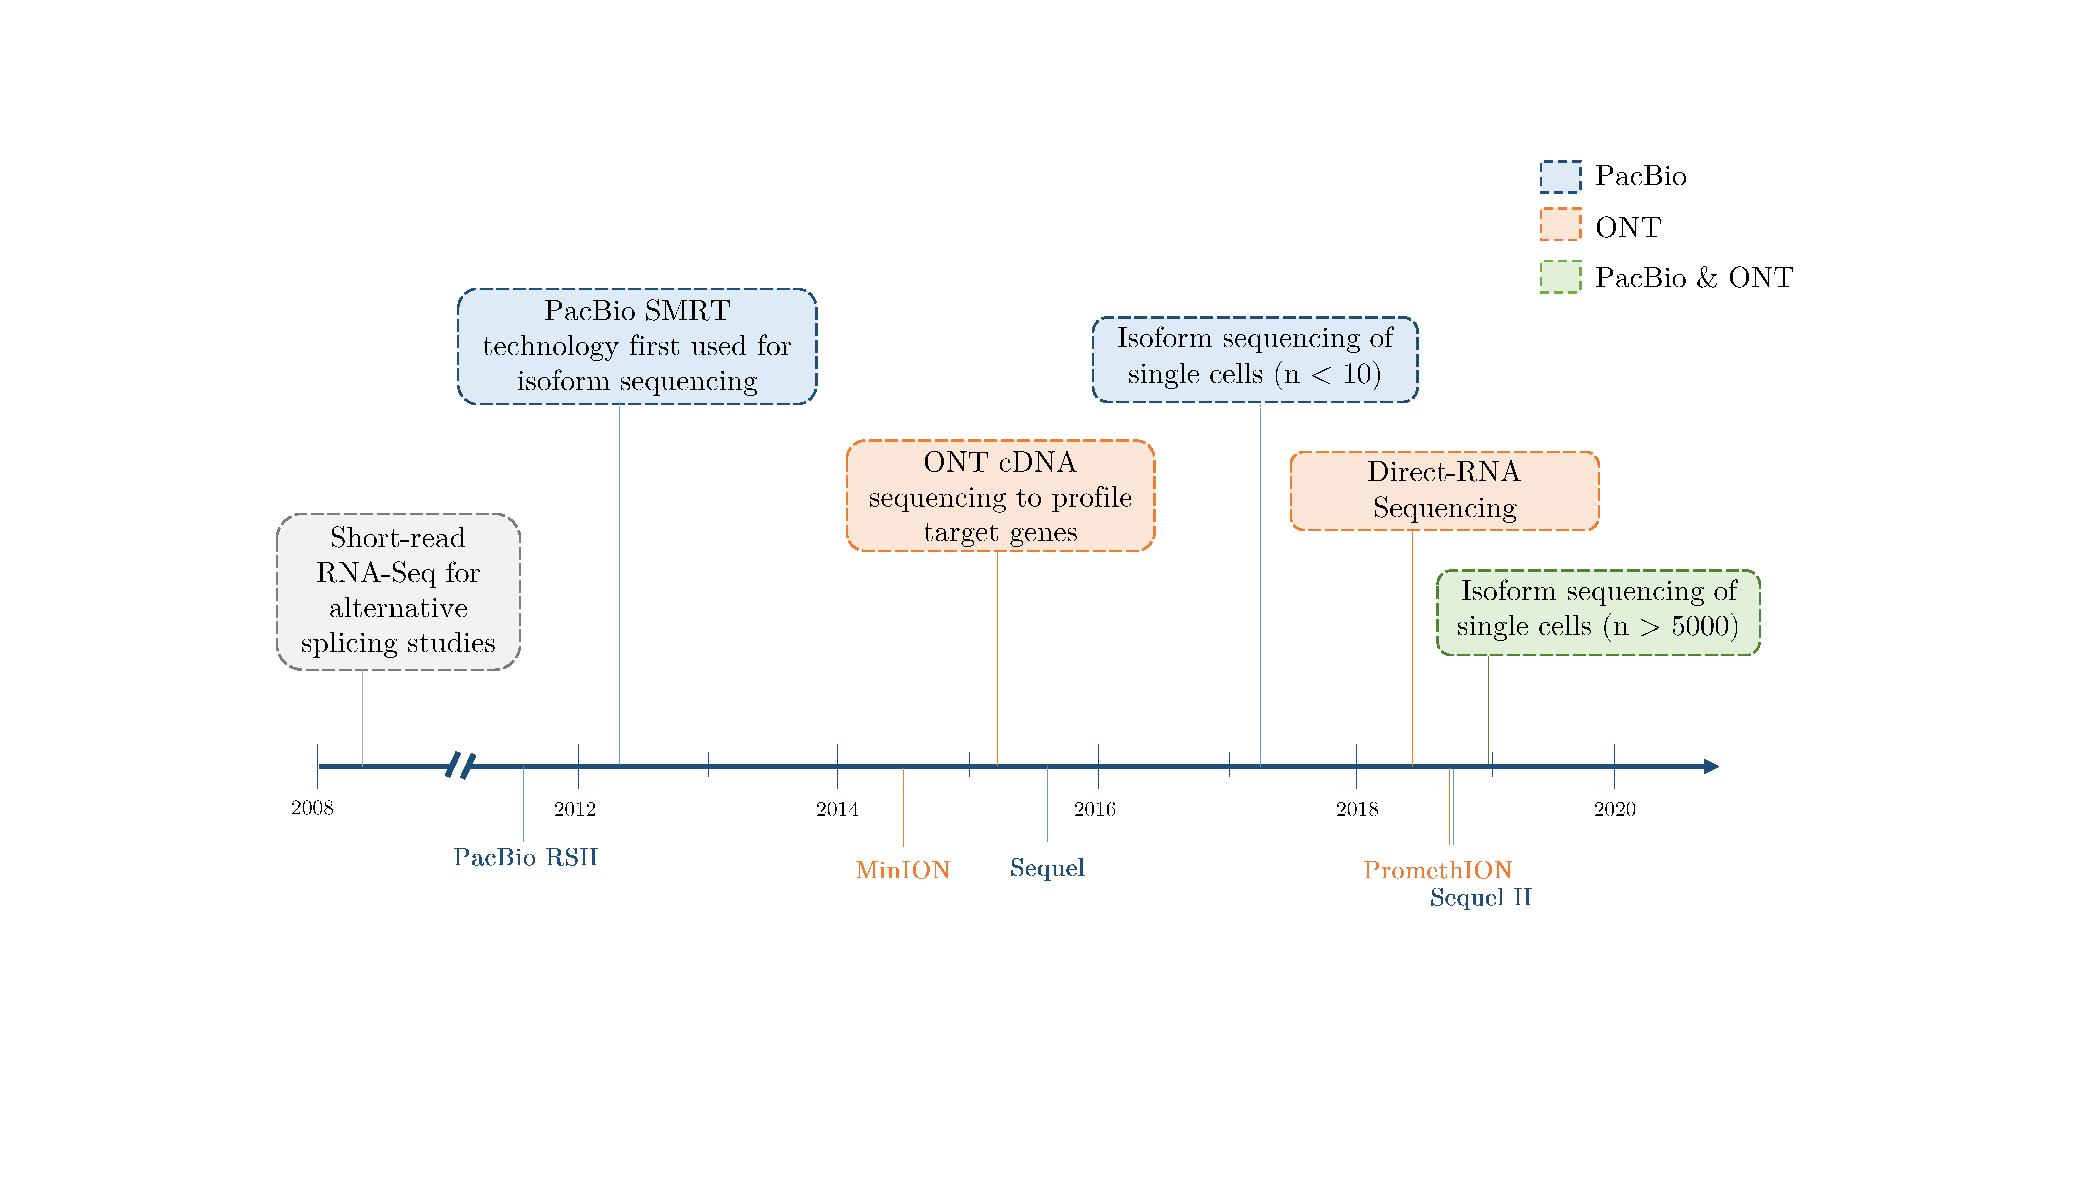
\includegraphics[page=1,trim={0 4cm 1.8cm 2cm},clip, scale = 0.8]{Figures/Introduction_Figures_Landscape.pdf}
			\captionsetup{margin={2cm,0cm}}
			\caption[Timeline of Long-read Sequencing Technologies \& Approaches]%
			{\textbf{Significant advances in long-read sequencing technology \& approaches.} Major breakthroughs in long-read sequencing approaches of isoforms using Pacific Bioscience's (PacBio) Single molecule real-time sequencing (SMRT) (boxed blue) and Oxford Nanopore sequencing (ONT, boxed orange) are highlighted. Release of respective technologies are also marked.}
			\label{fig:longread_timeline}
		\end{figure}
	\end{landscape}
	
	
	%\captionsetup{width=30cm}
	\begin{landscape}
		\small %smaller font
		\setlength\tabcolsep{2pt} %reduced margin size in table
		\renewcommand{\arraystretch}{1}
		\begin{longtable}[c]{p{4cm}p{4cm}p{18cm}}
			\caption[Advances in Long-read sequencing technologies: Single Cell and Direct RNA-Sequencing]%		
			{\textbf{Advances in Long-read sequencing technologies: Single Cell and Direct RNA-Sequencing}, DIE - differential isoform expression, ONT - Oxford Nanopore Technologies, SE - Skipped Exon, TSS - Transcription Start Site, TTS - Transcriptional Termination Site, }
			\label{tab: longread_advancedstudies}\\
			
			\toprule
			\multicolumn{1}{c}{References} &
			\multicolumn{1}{c}{Samples and Tissue} &
			\multicolumn{1}{c}{Key Findings} \\* \midrule
			\endfirsthead
			%
			\endhead
			%
			\bottomrule
			\endfoot
			%
			\endlastfoot
			%								
			\centering Karlsson \& Linnarsson (2017)\cite{Karlsson2017} &
			\centering Mouse single cels (n = 6)  &
			\tabitem High isoform diversity observed within single-cell oligodendrocytes with \textasciitilde1000 distinct isoforms mapped to 700 genes with low overlap between cells, predominantly driven by alternative TSS and TTS \\
			\hdashline[0.5pt/5pt]	
			
			\centering Gupta et al.(2018) \cite{Gupta2018} &
			\centering Mouse cerebellum (n = 1)  &
			\tabitem Long-read sequencing of >5000 single cells (microglia, astrocytes, neurons) after isolation \& barcoding \newline 
			\tabitem Identified cell-specific \textit{Bin1} isoforms with skipping of A1 and A2-A6 alternative exons (separated by constitutive exons) in all microglia, some astrocytes but not in neuronal cell-types, indicating cell-specific SE coordination \\
			\hdashline[0.5pt/5pt]			
			
			\centering Byrne et al. (2017)\cite{Byrne2017} &
			\centering Mouse single B1a cells (n = 7) &
			\tabitem Identified thousands of novel TSS and TTS (within 20bp bins due to lower error rate) \& hundreds of splicing events \newline
			\tabitem 160 genes with complex isoforms, 55 of which showed differential isoform usage (including B cell receptors) \\
			\hdashline[0.5pt/5pt]
			
			\centering Volden et al. (2018) \cite{Volden2018} &
			\centering Human single B cells (n = 96 from 1 donor) &
			\tabitem Circularising input cDNA and generating a CCS read (R2C2) significantly improved raw (316,000 cDNA reads at 94\% accuracy) and splice site accuracy (92\% vs ONT 1D raw reads at 80\%, Iso-Seq CCS reads at 97\%, based on SIRVs) \newline 
			\tabitem Ability to accurately demultiplex reads based on 7-8nt barcodes enabling mass sequencing of single cells with accurate gene quantification (strongly correlated with RNA-Seq, r = 0.79) and identification of cell-specific isoforms \\
			\hdashline[0.5pt/5pt]
			
			
			\centering Garalde et al. (2018) \cite{Garalde2018} &
			\centering Yeast \newline ERCC RNA-Spike in mix &
			\tabitem Direct RNA Sequencing of yeast poly(A) RNA achieved good coverage (2.8M reads vs 5.7M reads using ONT cDNA) with negligible effect on transcript length and GC content \newline 
			\tabitem Accurately identification of splice variants with no missing or novel exons from spike-in, and able to rudimentally discriminate RNA modification (m\textsuperscript{6}A, 5-mC) using trained datasets  \\
			
			\centering Workman et al. (2019) \cite{Workman2019a} &
			\centering Human B lymphocyte cell line (n = 30) &
			\tabitem Direct RNA-Sequencing of human cell line documented a high proportion (52.6\%) of novel isoforms \newline
			\tabitem High error rate (14\%) \& significant 5'truncation due to technical issues (rapid translocation through pore, signal artefacts from enzyme stalling or strand breaks), making it difficult to ascertain TSS \newline
			\tabitem Differences in poly(A) length distribution between mitochondrial and nuclear genes, and between different isoforms of the same gene (increase in polyA tail-lengths of intron-retaining isoforms) \\
			\hdashline[0.5pt/5pt]
			
			\centering Sessegolo et al. (2019) \cite{Sessegolo2019} &
			\centering Mouse brain \& liver \newline(n = 3) &
			\tabitem Benchmark study of Illumina RNA-Seq, ONT cDNA-Seq with/without 5'cap, \& ONT Direct RNA-Seq. \newline
			\tabitem Biased ONT cDNA-Seq of truncated transcripts with internal runs of poly(T) (15nt) due to cDNA synthesis; ONT RNA-Seq most accurately quantified gene expression using spike-in, followed by RNA-Seq, cDNA-Seq  \\
			\hdashline[0.5pt/5pt]
			
			\centering Singh et al. (2019) \cite{Singh2019} &
			\centering Human T- \& B-cell lines \newline Tumour \& paired lymph node (n = 1)  &
			\tabitem Novel sequencing method (RAGE-Seq) combining droplet-based scRNA-Seq with target capture ONT cDNA-Seq \newline 
			\tabitem Able to differentiate naive and mature B cells, and subpopulation by accurate identification of antigen receptor; track clonally related cells across tissues revealing cell-specific expression changes between tumour \& lymph node \\
			\hdashline[0.5pt/5pt]
			
			\centering Joglekar et al. 2021 \cite{Joglekar2021} &
			\centering Mouse hippocampus \& prefrontal cortex (n = 2) &
			\tabitem Identified $\tilde{400}$ DIE genes between brain regions using gene-wise test (nx2 table with isoform counts per gene), which was governed predominantly by splice variant changes in one single cell type \newline 
			\tabitem Spatial transcriptomics with Iso-Seq (Sl-ISO-Seq) confirmed localisation of brain-region specific DIE (exon-based). 
			\\* \bottomrule
		\end{longtable}

		\begin{longtable}[c]{p{4cm}p{4cm}p{18cm}}
			\caption[Single cell sequencing studies of human AD post-mortem brain tissues and AD mouse models]%		
			{\textbf{Single cell sequencing studies of human AD post-mortem brain tissues and AD mouse models}. ARM - Activated Response Microglia, DEG - Differentially Expressed Gene, DIE - Differential Isoform Expression, IRM - Interferon Response Microglia, scRNA-Seq - Single Cell RNA-Sequencing}
			\label{tab: longread_AD_advancedstudies}\\
			
			\toprule
			\multicolumn{1}{c}{References} &
			\multicolumn{1}{c}{Samples and Tissue} &
			\multicolumn{1}{c}{Key Findings} \\* \midrule
			\endfirsthead
			%
			\endhead
			%
			\bottomrule
			\endfoot
			%
			\endlastfoot
			%								
			\centering Keren-Shaul et. al (2017)\cite{Keren-Shaul2017} &
			\centering 5xFAD AD mouse model (1 - 8 months) &
			\tabitem Few isoforms shared between cells (7\%) highlighting the importance of scRNA-Seq \newline
			\tabitem Identified subsets of protective microglia (disease-associated microglia - DAM), with a characteristic transcriptional activation profile:  Trem2-independent manner that involves downregulation of microglia checkpoints, followed by activation of a Trem2-dependent program for upregulation of phagocytic-related genes, essential for A$\beta$ clearance  \\
			\hdashline[0.5pt/5pt]	
			
			\centering Frigerio et. al (2019)\cite{Frigerio2019} &
			\centering App\textsuperscript{NL-G-F}\newline AD mouse model  &
			\tabitem Two activated states (reactive) of microglia: i) activated response microglia (ARM) characterised by upregulated expression of immune cells, and ii) interferon response microglia (IRM) characterised by upregulated expression of innate immune response and interferon response pathway  \newline
			\tabitem ARM was enriched with GWAS AD risk genes: \textit{Trem2} upregulation, \textit{Bin1, Cd33, Picalm} downregulation  \newline
			\tabitem ARM promoted \textit{Apoe} expression in microglia, whereby deletion of \textit{Apoe} ablated ARM expression and density of microglia around amyloid deposits \\
			\hdashline[0.5pt/5pt]
			
			\centering Mathys et. al (2019)\cite{Mathys2019} &
			\centering Human Prefrontal Cortex (24 AD, 24 Controls)  &
			\tabitem Identified cell-specific response with upregulation of microglial-expressed genes (i.e. \textit{TREM2},\textit{PICALM}) \newline
			\tabitem 95\% of DEGs were observed in one cell type, indicating perturbations are strongly cell specific.  However, top DEGs enriched were in myelination across multiple cell types (i.e. \textit{ERBIN, CNTNAP2, NEGR1, BEX1, NTNG1} )   \\
			\hdashline[0.5pt/5pt]
			
			\centering Grubman et. al (2019)\cite{Grubman2019} &
			\centering Human Entorhinal Cortex (6 AD, 6 Controls)  &
			\tabitem \textit{APOE} is specifically repressed in oligodendrocyte progenitor cells and astrocyte subpopulations, while upregulated in microglial subpopulation  \\
			\hdashline[0.5pt/5pt]
			
			\centering Leng et. al (2021)\cite{Leng2021} &
			\centering AD Entorhinal Cortex (6 Control, 6 AD)  &
			\tabitem Subset of AD-associated astrocytes, likely to represent reactive astrocytes, characterised with upregulated expression of \textit{GFAP} and \textit{CD44}, and downregulation of genes associated with homeostasis  		
			\\* \bottomrule
		\end{longtable}
	\end{landscape}
\end{changemargin}


\newpage
\section{Aims and Objectives}
An increasing number of studies implicate a role of transcriptional dysregulation and aberrant splicing in AD disease development and pathogenesis (reviewed in \cref{tab: AS_ADHuman_studies}). However, investigation of splicing and transcript expression changes is typically performed by profiling the transcriptome using standard short-read RNA-Sequencing approaches, which are inherently-constrained at transcript assembly and subsequent isoform characterisation essential for splicing analysis (described in \cref{rnaseq_intro}). My PhD thus aims to overcome these challenges by leveraging the use of long-read sequencing to accurately characterise isoform diversity and splicing patterns associated with Alzheimer's disease (\cref{fig:studydesign}).

%Further limitations of RNA-Seq studies
%By identifying and characterising such alternative splicing events, there is hope of deepening current understanding of the biological role of transform isoform diversity and in the case of AD, identify novel pathways involved in pathogenesis of disease as potential target treatments. 

\textbf{Hypothesis}: Transcriptomic dysregulation plays a fundamental role in development of AD pathology. This includes alterations in gene splicing, which results in differential and novel expression of transcripts that are translated to generate isoforms with functional biological implications. 

\textbf{Main Objectives}:

\begin{enumerate}[]
	\item Optimise long-read sequencing approaches, PacBio Iso-Seq and ONT complementary DNA (cDNA)\nomenclature{cDNA}{Complementary DNA} nanopore sequencing, for profiling of full-length transcripts (\cref{ch: long_read_sequencing}) 
	\item Characterise global isoform diversity and splicing events in mouse cortex using optimised long-read sequencing approaches (\cref{ch: whole_transcriptome}) 
	\item Identify global transcriptional and splicing changes associated with progression of tau pathology using well-characterised AD mouse model, rTg4510 (\cref{ch: transcriptional_global_differences})
	\item Comprehensively characterise isoform diversity and splicing events of 20 AD-associated genes, and changes in transcript expression associated with tau pathology in rTg4510 mice (\cref{ch: targeted_transcriptome})
	\item Identify AD-associated differential splicing and transcript expression in human AD post-mortem brain tissue and relate findings to those identified in mouse (\cref{ch: BDR})
	\item Integrate transcriptomic analyses with epigenetic (\cref{ch: targeted_transcriptome}) and proteomic data (\cref{ch: BDR}), available from the same samples
\end{enumerate}
% Integrative Papers
% https://www.nature.com/articles/s41588-020-00773-z importance of linking genomics with proteomics
% https://www.nature.com/articles/s41591-020-0815-6 - more proteomics
% https://www.nature.com/articles/s41588-020-0696-0 - epigenetics


\begin{landscape}
	\begin{figure}[htb]
		\begin{center}
			\includegraphics[page=2,trim={0 0 0 0},clip,scale = 0.7]{Figures/Introduction_Figures_Landscape.pdf}
		\end{center}
		\captionsetup{width=1.5\textwidth}
		\caption[Study design and analysis overview]%
		{\textbf{Study design and analysis overview}. To identify transcriptomic and splicing changes associated with AD pathology, this thesis aims to characterise isoform diversity and splicing events at a global and targeted level from the rTg4510 mouse model and AD human post-mortem brain tissues. ONT - Oxford Nanopore Technology, PacBio Iso-Seq - Pacific Bioscience's Isoform Sequencing}
		\label{fig:studydesign}
	\end{figure} 	
\end{landscape}